\documentclass[12pt]{report}
\usepackage[margin=1cm, top=1.5cm, bottom=1.5cm]{geometry}
\usepackage{minted}
\usepackage{xcolor}
\usepackage{tcolorbox}
\usepackage{babel}
\usepackage[T1]{fontenc}
\usepackage{textcomp}
\usepackage{titlesec}
\usepackage[hidelinks]{hyperref}
\usepackage{bookmark}
\usepackage{tikz}
\usepackage{tabularx}
\usepackage{pdfpages}
\usepackage{float}
\usetikzlibrary{calc}
\tcbuselibrary{minted}


\renewcommand{\theFancyVerbLine}{\textcolor{gray!50}{\scriptsize\arabic{FancyVerbLine}}}
\renewcommand{\contentsname}{Tartalomjegyzék}

\definecolor{getColor}{HTML}{4CAF50}
\definecolor{postColor}{HTML}{2196F3}
\definecolor{patchColor}{HTML}{FF9800}
\definecolor{deleteColor}{HTML}{F44336}
\definecolor{putColor}{HTML}{9C27B0}

\newcommand{\httpGet}[1]{\colorbox{getColor}{\textbf{\textcolor{white}{GET}}}~#1}
\newcommand{\httpPost}[1]{\colorbox{postColor}{\textbf{\textcolor{white}{POST}}}~#1}
\newcommand{\httpPatch}[1]{\colorbox{patchColor}{\textbf{\textcolor{white}{PATCH}}}~#1}
\newcommand{\httpDelete}[1]{\colorbox{deleteColor}{\textbf{\textcolor{white}{DELETE}}}~#1}
\newcommand{\httpPut}[1]{\colorbox{putColor}{\textbf{\textcolor{white}{PUT}}}~#1}

\titleformat{\chapter}
  {\normalfont\Huge\bfseries}
  {\thechapter.}
  {0.5em}                      
  {} 

\newtcolorbox{codeblock}[2][]{
  colback=black!85!gray,
  colframe=black!50!gray, % Gradient effect
  colbacktitle=black!50!gray,
  coltitle=white,
  title={\ttfamily#2},
  fonttitle=\footnotesize\bfseries,
  arc=5pt,
  boxrule=1pt,
  toptitle=4pt,
  bottomtitle=2pt,
  left=25pt,
  right=5pt,
  top=2pt,
  bottom=2pt,
  % sharp corners=south,
  #1
}

\begin{document}

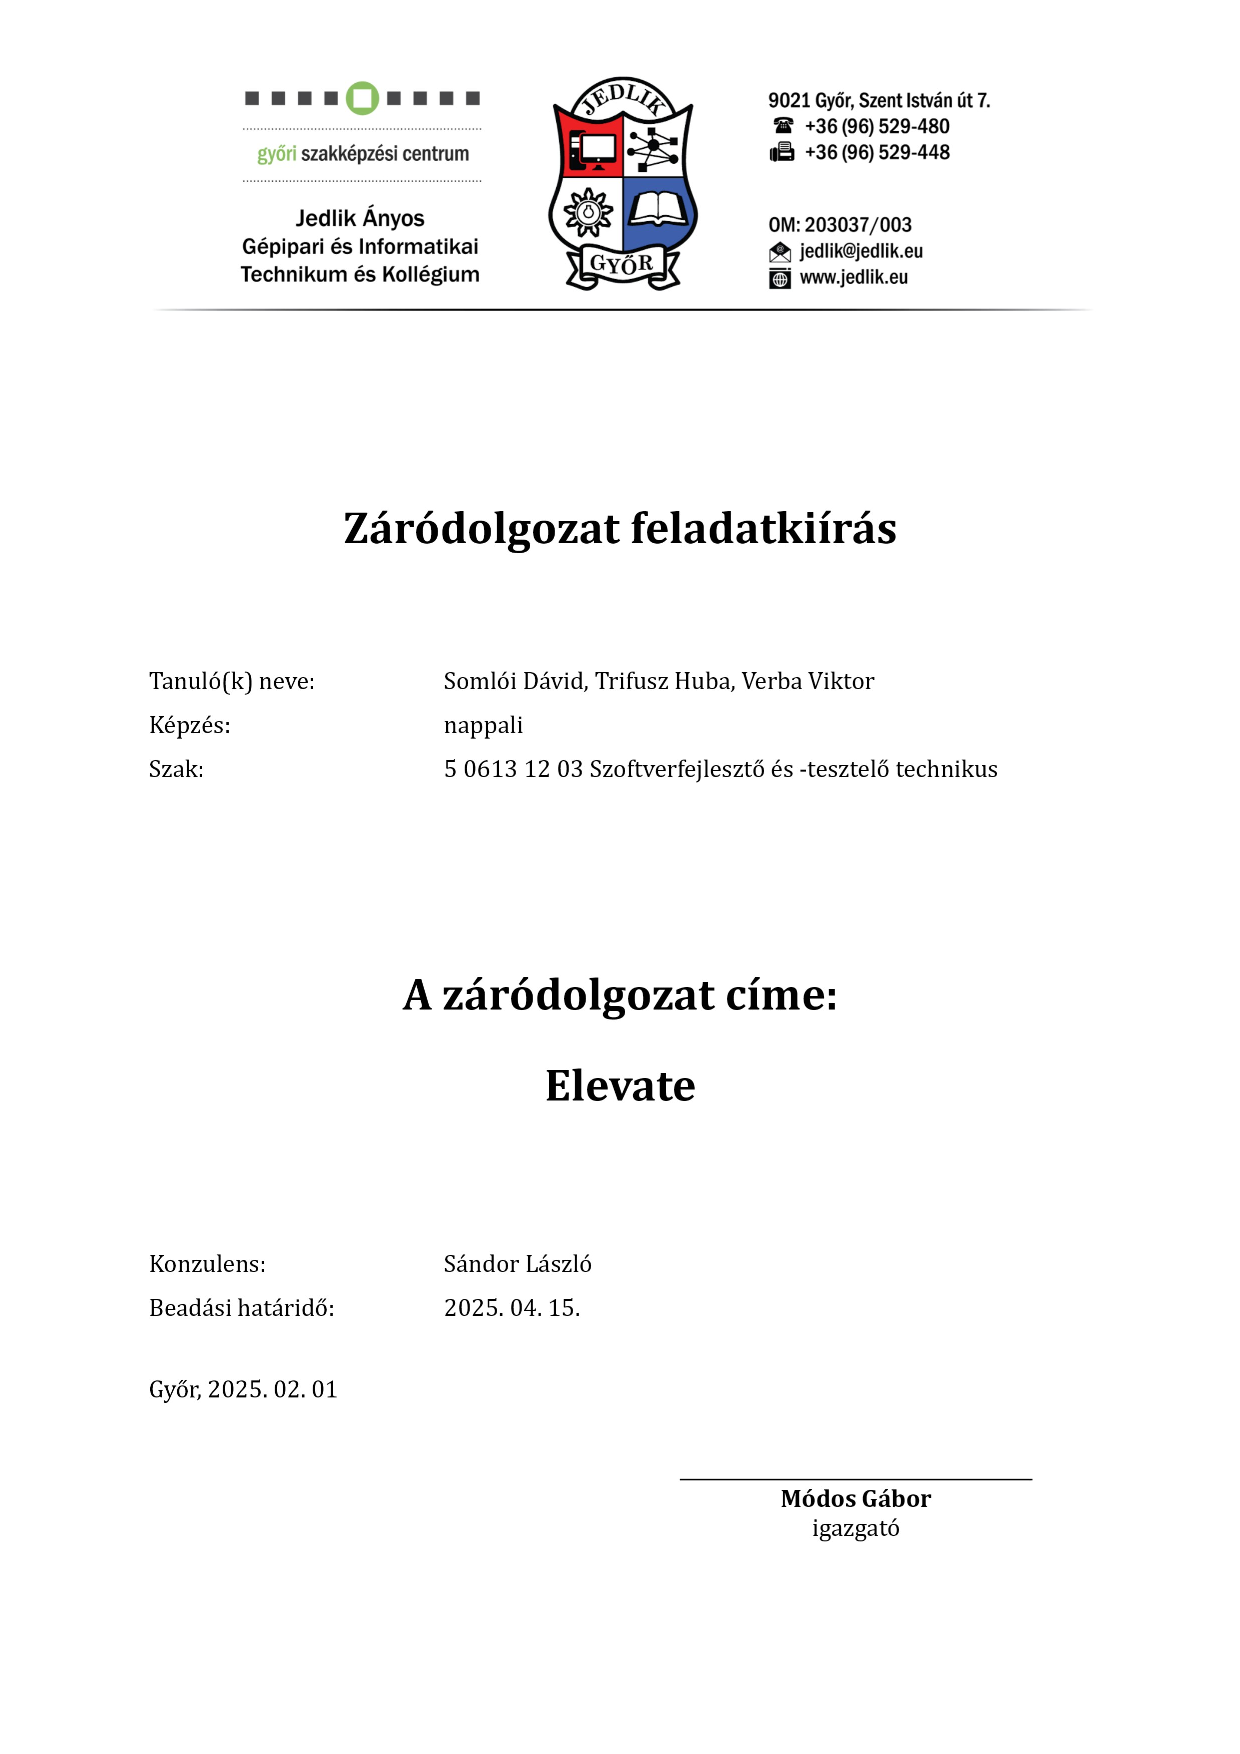
\includepdf[pages=-]{src/cover.pdf}

\setcounter{tocdepth}{2}
\tableofcontents

\chapter{A projektről}
\begin{sloppypar}
A téma kiválasztásánál arra törekedtünk, hogy egy, a hétköznapi élet során alkalmazható szoftvert készítsünk. Több opció is felmerült, azonban végül egy szokásformáló felület mellett döntöttünk, amit Elevate-nek neveztünk el, az egészséges, felemelő életmód jegyében. Az Elevate ösztönzi a felhasználókat, hogy új, pozitív szokásokat vezessenek be, miközben hatékonyan követhetik saját fejlődésüket, emellett hozzájárul életminőségük javításához és a fenntartható fejlődéshez.
\end{sloppypar}
\section{Az Elevate célja és funkciói}
\begin{sloppypar}
A szoftver célja, hogy a kliens az általa kívánt szokásokat fejlessze, vagy újakat építsen be a napirendjébe. Például, ha a felhasználó a dohányzásról szeretne leszokni, akkor monitorozni tudja a fogyasztását, nyomon követheti haladását a felálított célja felé. Nem csak a rossz szokások követését biztosítja az applikáció, pozitív célokat is ki lehet tűzni, mint “Napi 10 fekvőtámasz" vagy “Hetente kitakarítani”. Új szokásokat napi, heti, havi vagy egyéni rendszerességgel lehet felvenni. Az egyéni opció választása esetén a felhasználó megadhatja, hogy a hét melyik napjain szeretné elvégezni a feladatot. Egy szokás tartásához elengedhet-etlen, hogy a beállított gyakorisággal teljesítsük a kitűzött kihívásokat. Ennek megkönnyítése érdekében az Elevate egy naptárszerű nézetben, színkódolva jeleníti meg a teendőket és emlékeztet azok elvégzésére. Minden elvégzett feladat után növekedik az adott szokáshoz tartozó streakje, ezzel ösztönözve arra, hogy megszakítás nélkül, konzisztensen küzdjön a céljáért. Ezen felül barátokat is hozzáadhatunk, akikkel kihívásokat indíthatunk, így még inkább motiválva egymást a célok elérésére.
\end{sloppypar}
\section{Munkamegosztás}

A projekt során a csapattagok az alábbi feladatkörökért feleltek:

\begin{itemize}
  \item \textbf{Verba Viktor} -- Az alkalmazás mobilos változatának teljes körű fejlesztése, beleértve a felhasználói felületet és a funkcionális működést.
  
  \item \textbf{Somlói Dávid} -- A backend logika, az adatbázis tervezése és megvalósítása, valamint az API-k elkészítése és karbantartása.
  
  \item \textbf{Trifusz Huba} -- A webes frontend felület teljes körű fejlesztése, kialakítása, a funkcionális elemek implementálása.
\end{itemize}
\chapter{Weboldal}
A frontend fejlesztéséhez az \textbf{Angular} keretrendszert használtuk, amely lehetővé tette számunkra a dinamikus, reszponzív alkalmazás fejlesztését. Az alkalmazás felépítése \textbf{TypeScript} nyelven történt, amely biztosítja a típusellenőrzést és a fejlettebb fejlesztési lehetőségeket. A stílusokat \textbf{SCSS} segítségével alakítottuk ki, amely rugalmas és karbantartható megoldást biztosított, valamint elősegítette a könnyebb skálázást és az átláthatóbb kódot.
\section{Projekt Beállítása}

\subsection{Előfeltételek}
A projekt futtatásához szükséges előfeltételek, eszközök:
\begin{verbatim}
- Node.js (>= 14.x)
- npm (>= 6.x)
\end{verbatim}

\subsection{Telepítés}
\begin{enumerate}
    \item Klónozd a repozitóriumot:
    \begin{verbatim}
    git clone https://github.com/hubatrifusz/elevate.git
    \end{verbatim}
    
    \item Telepítsd a függőségeket:
    \begin{verbatim}
    cd elevate
    cd web-frontend
    npm install
    \end{verbatim}
    
    \item Indítsd el a fejlesztői szervert:
    \begin{verbatim}
    ng serve -o
    \end{verbatim}
    Az alkalmazás elérhető lesz a \texttt{http://localhost:4200} címen
\end{enumerate}

\newpage
\section{Mappastruktúra}
\subsection{Áttekintés a mappastruktúráról}
\begin{verbatim}
/web-frontend
 |-- /public           # Publikus fájlok (pl. képek)
 |-- /src             
 |   |-- /components   # Újrahasználható UI komponensek
 |   |-- /guards       # Biztonsági őrök (pl. autentikáció)
 |   |-- /models       # Adatmodellek
 |   |-- /pages        # Oldal komponensek (pl. HomePage, Dashboard)
 |   |-- /services     # API hívások és üzleti logika
 |   |-- index.html    # Alkalmazás belépési pontja
 |   |-- main.ts       # Alkalmazás belépési pontja
 |   |-- styles.scss   # Globális stílusok
 |-- /assets           # Statikus fájlok (pl. képek, betűtípusok)
 |   |-- /fonts        # Betűtípusok
 |   |-- /styles       # Stílus fájlok
 |-- /environments     # Környezeti konfigurációk
 |   |-- environment.ts
 |-- angular.json      # Angular konfigurációs fájl
 |-- package.json      # Projekt metaadatok és függőségek
\end{verbatim}

\section{Design és Prototípus Készítés}

A felhasználói felület és a design prototípusának elkészítéséhez \textbf{Figma} eszközt használtunk. A Figma lehetővé tette számunkra, hogy gyorsan és hatékonyan tervezzük meg az alkalmazás vizuális megjelenését, miközben valós időben együtt dolgozhattunk a csapat tagjaival. A design folyamat során interaktív prototípusokat készítettünk, amelyek segítettek a felhasználói élmény finomhangolásában, és biztosították a fejlesztés szoros összhangját a kívánt felhasználói élménnyel.

\section{Oldalak}
\subsection{Dashboard}

\subsubsection{Leírás}
A Dashboard oldal a felhasználó napi teendőit és a negatív szokásokat jeleníti meg.

\subsubsection{Fő komponensek}

\begin{itemize}
  \item \textbf{Task View} -- A napi feladatok listázása, új szokások felvétele, meglévő szokások törlése vagy módosítása.
  \item \textbf{Negative Habits} -- (külön komponens, részletezése később következik).
\end{itemize}

\subsubsection{Task View funkciói}

\begin{itemize}
  \item \textbf{Napi dátum kezelése} -- A felhasználó az aktuális, előző vagy következő napra navigálhat.
  \item \textbf{Napi szokások listázása} -- A mai napra rögzített szokások megjelenítése.
  \item \textbf{Új szokás hozzáadása} -- Pozitív vagy negatív szokás rögzítése űrlapon keresztül.
  \item \textbf{Szokások törlése és módosítása} -- A meglévő szokások frissítése vagy eltávolítása.
\end{itemize}

\subsubsection{Task komponens (Pozitív szokás)}

A napi feladatokat az \texttt{TaskComponent} jeleníti meg. Ez a komponens a következőket tartalmazza:

\begin{itemize}
  \item \textbf{Feladat bejelölése} -- A felhasználó checkbox segítségével jelezheti, hogy teljesítette-e az adott szokást.
  \item \textbf{Szokás adatok} -- A cím, leírás, szín és aktuális streak megjelenítése.
  \item \textbf{Leírás részletezése} -- Az egyes szokásokhoz tartozó részletes leírás lenyitható.
  \item \textbf{Jegyzet mentése} -- A felhasználó személyes jegyzeteket fűzhet a napi szokásnaplóhoz.
  \item \textbf{Állapot frissítése} -- A szokás teljesítésekor a feladat stílusa inaktívvá válik, és a streak számláló növekszik.
\end{itemize}

A komponens működése:
\begin{itemize}
  \item Ha a feladatot bejelölik, a háttér szín halványodik és egy API hívás történik a napló frissítésére.
  \item Ha a felhasználó megváltoztatja a jegyzetet, mentésre kerül az adatbázisba.
  \item A feladat részletei külön gomb segítségével lenyithatók vagy bezárhatók.
\end{itemize}

\subsubsection{Űrlap mezők}

\begin{itemize}
  \item Cím (kötelező)
  \item Leírás (kötelező)
  \item Színválasztás (kötelező)
  \item Pozitív/negatív szokás megkülönböztetése
  \item Gyakoriság kiválasztása (pozitív szokásoknál kötelező)
\end{itemize}

\subsubsection{Állapotok kezelése}

\begin{itemize}
  \item Új szokás létrehozása sikeres vagy sikertelen esetén figyelmeztető üzenetet jelenít meg.
  \item Betöltés közbeni spinner animáció.
  \item Üres napi lista esetén: ``No tasks for today!'' üzenet megjelenítése.
\end{itemize}

\subsubsection{Negative Habits (Negatív szokások)}

A negatív szokásokat a \texttt{NegativeHabitsComponent} kezeli. Minden negatív szokás egy külön \texttt{NegativeHabitComponent} komponensben jelenik meg.

\begin{itemize}
  \item \textbf{Lista betöltése} -- A felhasználó negatív szokásai lekérésre kerülnek a szerverről.
  \item \textbf{Napok számlálása} -- Minden szokás esetén látható, hogy hány nap telt el az utolsó visszaesés óta.
  \item \textbf{Kördiagram megjelenítése} -- A napok számát arányosan kitöltött színes körgrafika ábrázolja.
  \item \textbf{Automatikus frissítés} -- A számláló 10 percenként automatikusan újraszámolódik.
\end{itemize}

A kördiagram kitöltésének logikája:
\begin{itemize}
  \item A háttér egy \texttt{conic-gradient} segítségével töltődik ki.
  \item A kitöltés aránya: \texttt{differenceInDays / 3.65 \%}.
\end{itemize}

 \subsection{Friends}

\subsubsection{Leírás}
A Barátok oldal lehetőséget ad:
\begin{itemize}
  \item Barátok keresésére e-mail cím alapján
  \item Barátkérések elfogadására vagy elutasítására
  \item Barátok törlésére
  \item Barátok listájának megtekintésére
\end{itemize}

\subsubsection{Függvények}

\begin{itemize}
  \item \textbf{searchUsers()} -- Felhasználók keresése e-mail cím alapján.
  \item \textbf{getFriends()} -- Barátok lekérése az adatbázisból.
  \item \textbf{sendFriendsRequest(friendId, event)} -- Barátkérés küldése egy másik felhasználónak.
  \item \textbf{getFriendRequests()} -- Beérkezett barátkérések lekérése.
  \item \textbf{getSentFriendRequests()} -- Elküldött barátkérések lekérése.
  \item \textbf{acceptFriendRequest(friend)} -- Barátkérés elfogadása.
  \item \textbf{declineFriendRequest(friend)} -- Barátkérés elutasítása.
  \item \textbf{deleteFriend(friend)} -- Barát törlése a listából.
  \item \textbf{showOptions(event, friend)} -- Opciók megjelenítése (pl. törlés gomb).
  \item \textbf{hideOptions(event)} -- Opciók elrejtése kattintásra.
\end{itemize}

\subsection{Habits}

\subsubsection{Leírás}
A Szokások oldal segítségével a felhasználók kezelhetik saját szokásaikat, kihívásokat küldhetnek barátoknak, elfogadhatják vagy visszautasíthatják a kihívásokat.

\subsubsection{Függvények}

\begin{itemize}
  \item \textbf{ngOnInit()} -- A komponens inicializálása, szokások és kihívások betöltése.
  \item \textbf{loadHabits()} -- A felhasználó szokásainak lekérése és megjelenítése.
  \item \textbf{loadChallengeInvites()} -- A felhasználónak érkezett kihívások lekérése.
  \item \textbf{openChallengeModal(habit)} -- Kihívás küldési modal ablak megnyitása adott szokásnál.
  \item \textbf{closeChallengeModal()} -- A kihívásküldő modal bezárása.
  \item \textbf{challengeFriend(friendId)} -- Kihívás küldése egy barátnak egy szokás alapján.
  \item \textbf{acceptChallenge(challenge)} -- Egy beérkezett kihívás elfogadása.
  \item \textbf{declineChallenge(challenge)} -- Egy beérkezett kihívás visszautasítása.
  \item \textbf{isFriendAlreadyChallenged(friendId)} -- Ellenőrzi, hogy egy barát már ki lett-e hívva adott szokásra.
  \item \textbf{isHabitOwner(habit)} -- Ellenőrzi, hogy a szokás tulajdonosa-e a bejelentkezett felhasználó.
  \item \textbf{deleteHabit(habit)} -- Egy szokás törlése a listából.
\end{itemize}

\subsection{Feed}

\subsubsection{Leírás}
A Feed oldal publikus posztokat jelenít meg a felhasználók számára. Ha nincsenek elérhető posztok, azt üzenetben jelzi.

\subsubsection{Függvények}

\begin{itemize}
  \item \textbf{constructor()} -- A komponens inicializálásakor automatikusan meghívja a feed betöltését.
  \item \textbf{loadFeed()} -- Lekéri az aktuális felhasználó számára elérhető publikus posztokat. Hiba esetén kezeli az üres feed állapotát.
\end{itemize}


\section{Komponensek}

\subsection{Áttekintés}

\textbf{Újrahasználható Komponensek}: A projektben számos újrahasználható komponens található, amelyek a különböző oldalakon és funkciókban alkalmazhatók, hogy javítsák a kód újrahasználhatóságát, karbantarthatóságát és olvashatóságát. Ilyen komponensek például:

\begin{itemize}
  \item \textbf{Loading spinner}: Egy betöltési animáció, amely jelzi, hogy az alkalmazás adatokat tölt be vagy folyamatban lévő műveletet végez.
  \item \textbf{Validation message}: Egy üzenetkomponens, amely tájékoztatja a felhasználót a hibás adatokkal kapcsolatban, például hiányzó mezők vagy érvénytelen formátum esetén.
  \item \textbf{Navbar}: Egy navigációs sáv, amely lehetővé teszi a felhasználó számára a különböző oldalakon való navigálást.
\end{itemize}

\textbf{Oldal Komponensek}: Ezek a komponensek az alkalmazás egyes oldalaihoz tartoznak. Minden oldalhoz saját komponens tartozik, amelyek kezelik a megjelenítést és a dinamikus adatokat. Részletesebben feljebb lehet őket megtekinteni. Példák:

\begin{itemize}
  \item \textbf{Dashboard}: A felhasználói irányítópult komponense, amely összegzi az alkalmazás legfontosabb információit.
  \item \textbf{Habits}: A felhasználó pozitív és negatív szokásait megjelenítő és kezelő oldal.
\end{itemize}

\subsection{Funkcionalitás}

\subsubsection{Fő Funkciók}
\begin{itemize}
  \item \textbf{Felhasználói Hitelesítés}: A felhasználó hitelesítése a rendszerbe való belépéskor történik. Az alkalmazás a bejelentkezés és a regisztráció során JWT tokeneket használ, hogy biztosítsa a felhasználó hitelesítését és jogosultságát.
  \item \textbf{Űrlapok kezelése}: A szokások hozzáadásához és módosításához űrlapokat használunk, amelyek tartalmazzák a szokás címét, leírását, színválasztását és egyéb paramétereket. Az űrlap validálása Angular form-control segítségével történik. A sikeres vagy sikertelen műveletek érdekében hibakezelés és figyelmeztető üzenetek is megjelennek.
  \item \textbf{API Integráció}: Az API hívásokat az Angular szolgáltatásain keresztül kezeljük. Az Angular beépített HTTP modulját használjuk az API-k elérésére. A \texttt{UserService} és \texttt{HabitService} szolgáltatások segítségével történnek a felhasználói és szokásadatok lekérése és frissítése.
  \item \textbf{Állapotkezelés}: Az alkalmazás állapotát az Angular szolgáltatások kezelik, amelyek az adatokat és a felhasználói interakciókat menedzselik. A \texttt{UserService} és \texttt{HabitService} biztosítják, hogy a felhasználói és szokás adatokat a komponensek között megfelelően osszuk meg. Az állapot frissítése minden interakció során automatikusan megtörténik, és a komponensek az Angular változásfigyelő mechanizmusain keresztül frissülnek.
\end{itemize}

\subsubsection{API Hívás Példa}

API hívások az Angular HTTP Client használatával:

\begin{codeblock}{HabitService.ts}
  \inputminted[
    style=one-dark,
    breaklines,
    linenos,
    firstline=13,
    lastline=34
  ]{typescript}{/home/smapesz/code/elevate/web-frontend/src/app/services/habit.service.ts}
\end{codeblock}



A fenti kód segítségével történnek az API hívások az \texttt{HttpClient} modulon keresztül. A \texttt{getHabits()} metódus lekéri a szokásokat, míg a \texttt{updateHabitLog()} frissíti a meglévő szokás adatokat.


\section{Stílusok}

A projekt stílusait SCSS fájlokban definiáljuk, hogy rugalmasan kezelhessük a különböző megjelenési elemeket, mint például a színeket, betűméreteket és elrendezéseket. Az alábbiakban bemutatásra kerülnek a legfontosabb változók és stílusok, amelyek az alkalmazás kinézetét meghatározzák.

\subsection{Változók (variables.scss)}

A stílusok alapja a \texttt{variables.scss} fájlban található változók, amelyek a különböző színeket, betűméreteket, valamint az alapvető dimenziókat tartalmazzák.

\subsubsection{Színek}
A színek különböző kategóriákra vannak bontva, mint például az akcentus színek, fő színek, szövegszínek, figyelmeztető színek és feladat színek:

\begin{itemize}
    \item \textbf{Akcentus színek:} A projekthez használt hangsúlyos színek, mint például \texttt{\$accent-color-100}, \texttt{\$accent-color-200} stb.
    \item \textbf{Fő színek:} A háttérszínek, mint például \texttt{\$main-color-100}, \texttt{\$main-color-200} stb.
    \item \textbf{Szövegszínek:} A szövegekhez használt színek, például \texttt{\$text-color-100}, \texttt{\$text-color-200} stb.
    \item \textbf{Figyelmeztető színek:} A hibák és figyelmeztetések megjelenítéséhez használt színek, mint például \texttt{\$alert-color-100}, \texttt{\$alert-color-200} stb.
    \item \textbf{Feladat színek:} A különböző típusú feladatokhoz rendelt színek, mint például \texttt{\$task-color-red}, \texttt{\$task-color-blue}, \texttt{\$task-color-green}.
\end{itemize}

\subsubsection{Betűtípusok és Méretek}
A \texttt{variables.scss} fájlban található a projekt által használt betűtípusok és betűméretek definíciója is:

\begin{itemize}
    \item \textbf{Betűtípus:} Az \texttt{Inter} betűtípus van használatban, amely a következő módon van importálva:
    \begin{verbatim}
    @font-face {
        font-family: 'Inter';
        src: url('../fonts/Inter-VariableFont_opsz\,wght.ttf') format('truetype');
    }
    \end{verbatim}
    \item \textbf{Betűméretek:} A különböző szövegekhez rendelt betűméretek a következők:
    \begin{itemize}
        \item \texttt{\$font-size-xs: 12px;}
        \item \texttt{\$font-size-sm: 14px;}
        \item \texttt{\$font-size-base: 16px;}
        \item \texttt{\$font-size-md: 18px;}
        \item \texttt{\$font-size-lg: 20px;}
        \item \texttt{\$font-size-xl: 24px;}
        \item \texttt{\$font-size-2xl: 32px;}
        \item \texttt{\$font-size-3xl: 48px;}
    \end{itemize}
\end{itemize}

\subsubsection{Dimenziók}
A különböző méretek, például a szélességek, magasságok és a határok is a \texttt{variables.scss} fájlban találhatóak:

\begin{itemize}
    \item \texttt{\$sidebar\_width: 5rem;}
    \item \texttt{\$border\_radius: 10px;}
    \item \texttt{\$input\_height: 2rem;}
\end{itemize}

\subsection{Űrlapok és Input Mezök (inputs.scss)}

Az alkalmazásban az űrlapok és bemeneti mezők stílusait az \texttt{inputs.scss} fájlban definiáljuk. A bemeneti mezők, mint például a szöveg-, email-, jelszó-, kereső- és szövegdobozok egyedi stílusokat kaptak.

\subsubsection{Input Mezők}
A bemeneti mezők általános stílusai a következőképpen vannak megadva:

\begin{itemize}
    \item A mezők háttérszíne \texttt{\$main-color-100}, a szöveg színe pedig \texttt{\$text-color-900}.
    \item A mezők határvonalai \texttt{\$main-color-600} színűek, és a mezők lekerekítettek \texttt{\$border\_radius} értékkel.
    \item A mezők fókuszálásakor a határvonal \texttt{\$accent-color-400}-ra változik, és az éppen kitöltött mezők címkéje átméreteződik és a \texttt{\$accent-color-400} színre vált.
    \item A checkbox inputok egyedi vizuális stílust kaptak, és csak akkor jelenítenek meg egy pipát, ha az adott checkbox be van jelölve.
\end{itemize}

\subsubsection{Feladatok Stílusai (task component)}
A feladatok megjelenítése a következő stílusokkal van definiálva az \texttt{task\_container} osztályban:

\begin{itemize}
    \item A feladatok konténere \texttt{display: flex;} és \texttt{flex-direction: column;} beállításokkal van struktúrába rendezve.
    \item A feladatok tetején található fejlécek a \texttt{task\_header\_container} osztályban vannak elhelyezve, amely tartalmazza a bal és jobb oldali információkat. A színük a \texttt{\$main-color-100} háttérszínt kapja, a szövegek színe pedig \texttt{\$text-color-900}.
    \item A feladatok részletei a \texttt{task\_details\_container} osztályban jelennek meg, amely az animációs hatásokkal bővített magasságot használ.
    \item A feladatokhoz kapcsolódó nem mai szokások esetén egy egyszerű stílusú cím és határidő jelenik meg, amelyek szintén a változókkal vannak testreszabva.
\end{itemize}


\chapter{Mobil Applikáció}
\section{Technológia}
Az Elevate mobilalkalmazása Ionic keretrendszerre épül, amely Angular alapú. Ez a kombináció lehetővé teszi a cross-platform fejlesztést, így egyetlen kódbázisból készíthető el az Android és iOS platformokra optimalizált alkalmazás. A felhasználói felület az Ionic komponenskönyvtárát és egyedi SCSS stílusokat használ. A backend API-val való kommunikáció Angular HttpClient-en keresztül történik.

\section{Architektúra}
Az alkalmazás a következő fő komponensekből épül fel:
\begin{itemize}
  \item \textbf{Modulok} - Az alkalmazás funkcionális egységei
  \item \textbf{Komponensek} - Újrafelhasználható UI elemek
  \item \textbf{Oldalak} - Az alkalmazás különböző képernyői
  \item \textbf{Service-k} - Üzleti logika és adatkezelés
  \item \textbf{Modellek} - Az adatstruktúrák TypeScript interfészei
  \item \textbf{Stílusok} - SCSS fájlok a megjelenés testreszabásához
  \item \textbf{Capacitor plugin-ok} - Natív funkciók elérése (kamera, értesítések)
\end{itemize}

\section{Mappastruktúra}
Az Elevate mobilalkalmazás a következő mappastruktúrával rendelkezik:

\begin{figure}
    \centering
    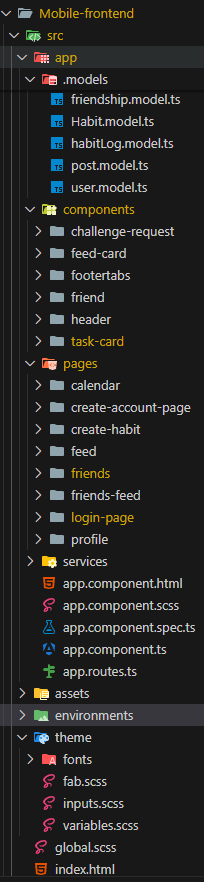
\includegraphics[width=0.11\linewidth]{src/mappastruktura.png}
    \caption{Mappastruktúra}
    \label{fig:enter-label}
\end{figure}

\textbf{Fő komponensek leírása:}
\begin{itemize}
  \item \textbf{components/} - Újrafelhasználható UI komponensek, amelyek több oldalon is megjelenhetnek (pl. szokás kártya, feed kártya)
  \item \textbf{models/} - TypeScript interfészek, amelyek az alkalmazásban használt adatstruktúrákat definiálják
  \item \textbf{pages/} - Az alkalmazás fő képernyői, minden képernyőhöz tartozik egy Angular komponens
  \item \textbf{services/} - A backend API-val való kommunikációt és egyéb adatkezelési funkciókat megvalósító szolgáltatások
  \item \textbf{guards/} - Útvonalvédelem, amely ellenőrzi a felhasználó jogosultságait az oldalak megtekintéséhez
\end{itemize}

\section{Főbb funkciók}
Az Elevate mobilalkalmazás a következő fő funkciókat kínálja:

\textbf{Autentikáció:}
\begin{itemize}
  \item Felhasználói regisztráció validációval (jelszó erősség ellenőrzés)
  \item Bejelentkezés JWT token alapú hitelesítéssel
  \item Profilkezelés (profilkép feltöltése)
\end{itemize}

\textbf{Szokáskövetés:}
\begin{itemize}
  \item Új szokások létrehozása 
  \item Szokások személyre szabása (cím, leírás, szín, gyakoriság)
  \item Egyedi gyakoriság beállítása (napok kiválasztása)
  \item Napi szokások megjelenítése és teljesítésük követése
  \item Sorozatok (streak) nyilvántartása és vizualizálása
\end{itemize}

\textbf{Feed és közösségi funkciók:}
\begin{itemize}
  \item Barátok tevékenységeinek követése
  \item Barátkérelmek kezelése
  \item Kihívások küldése és fogadása
  \item Felhasználók keresése
\end{itemize}

\textbf{Naptár nézet:}
\begin{itemize}
  \item Aznap teljesítendő szokások követése
  \item Jövőbeli szokások előnézete
\end{itemize}

\section{Felhasználói élmény és dizájn}
Az alkalmazás felhasználói felülete a következő alapelvekre épül:
\begin{itemize}
  \item \textbf{Reszponzív dizájn} - Alkalmazkodik különböző képernyőméretekhez
  \item \textbf{Sötét/világos téma} - Automatikus váltás a rendszerbeállítások alapján
  \item \textbf{Intuitív navigáció} - Alsó tabbar és oldalmenü kombinációja
  \item \textbf{Vizuális visszajelzések} - Animációk és toast üzenetek
  \item \textbf{Egyszerű űrlapok} - Validáció és hibaüzenetek
\end{itemize}

Az alkalmazás a Material Design elveit követi, egyedi színpalettával és tipográfiával kiegészítve. A fő színséma lila és kék árnyalatokra épül, ami a motivációt és a fejlődést szimbolizálja.


\section{Natív integráció}
A Capacitor segítségével az alkalmazás hozzáfér a készülék natív funkcióihoz:
\begin{itemize}
  \item Kamera használata profilképek készítéséhez
  \item Eszköztéma-követés (sötét/világos mód)
\end{itemize}

\section{Biztonság}
Az alkalmazás biztonsági szempontjai:
\begin{itemize}
  \item JWT token tárolása biztonságos módon
  \item Input validáció kliens oldalon
  \item Jelszavak biztonságos kezelése (minimális követelmények: 12 karakter, nagybetű, szám, speciális karakter)
  \item Nem autentikált felhasználók átirányítása a bejelentkezési oldalra
\end{itemize}

\section{Teljesítmény optimalizálás}
Az alkalmazás teljesítményét javító technikák:
\begin{itemize}
  \item Lazy loading az oldalak betöltéséhez
  \item Infinite scroll a hosszú listák kezeléséhez
  \item Képek optimalizálása
  \item Standalone komponensek használata
\end{itemize}

\chapter{Adatbázis}
\section{Adatbázis tervezés}
Az Elevate két különböző adatbázis rendszert támogat a különböző környezetekben való futtatáshoz:
\begin{itemize}
  \item Fejlesztési környezetben: MySQL
  \item Production környezetben: PostgreSQL
\end{itemize}

Erre azért van így, mert a fejlesztést MySQL-el kezdtük, majd a Koyeb-re való publikáláshoz szükségessé vált PostgreSQL kompatibilitás. Az adatbázis migrációk kezelésére az Entity Framework Core migrációs rendszerét használjuk, amely lehetővé teszi a séma verziókövetését és az adatbázis automatikus frissítését, ez kisebb módosításokkal mindkét adatbázis környezettel megfelelően működik.

\section{Entitások és kapcsolatok}
Az adatbázis séma a következő fő táblákat tartalmazza:

\begin{figure}[H]
    \centering
    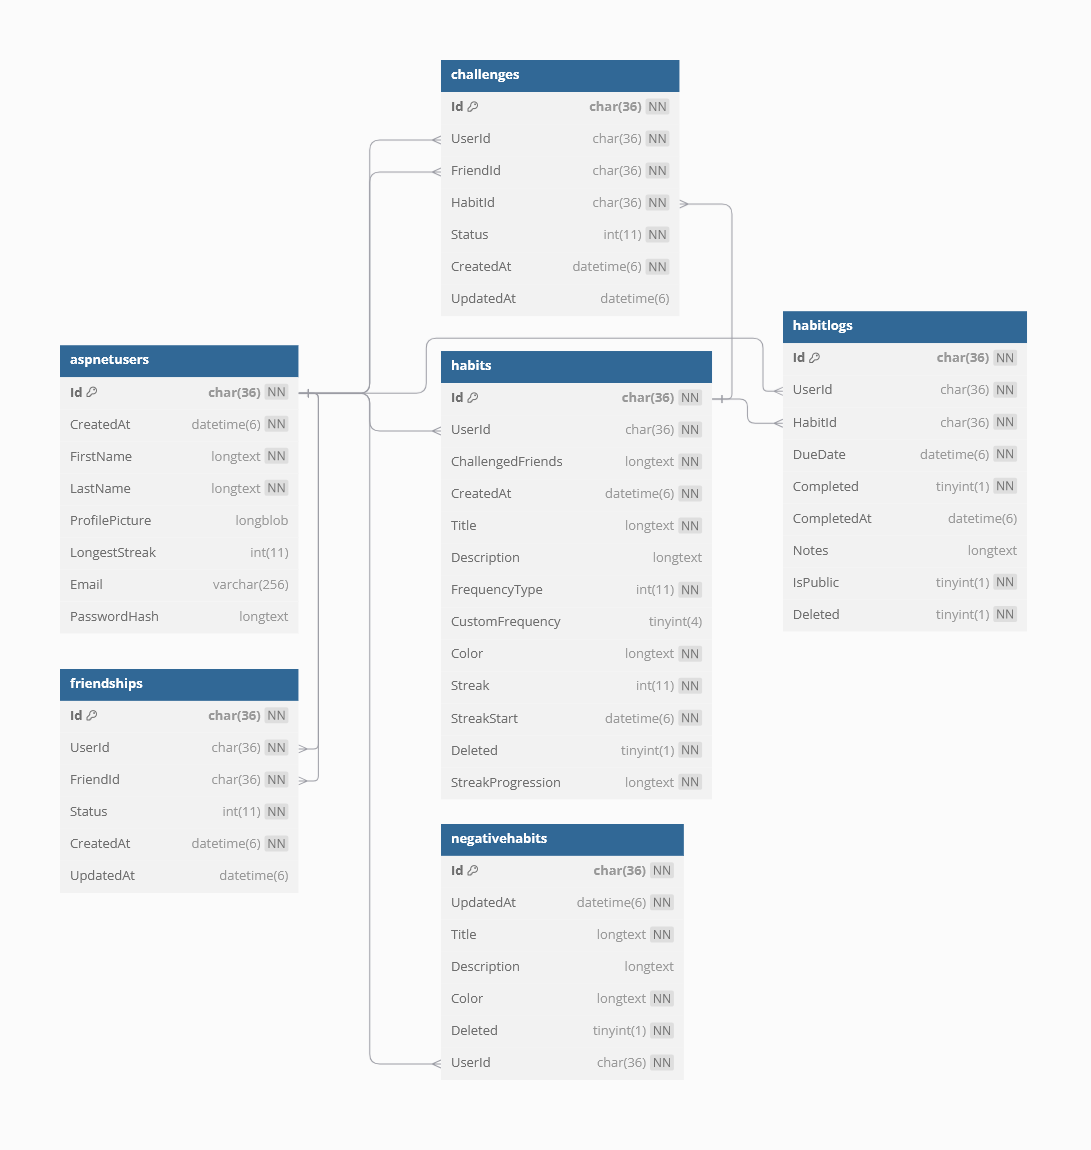
\includegraphics[width=0.5\textwidth, height=0.5\textheight, keepaspectratio]{src/diagram_min.png}
\end{figure}

Emellett az ASP.NET Core Identity által biztosított felhasználói táblák is megtalálhatóak, amelyek a felhasználók kezeléséért felelősek. A teljes adatbázis séma így néz ki:

\begin{figure}[H]
    \centering
    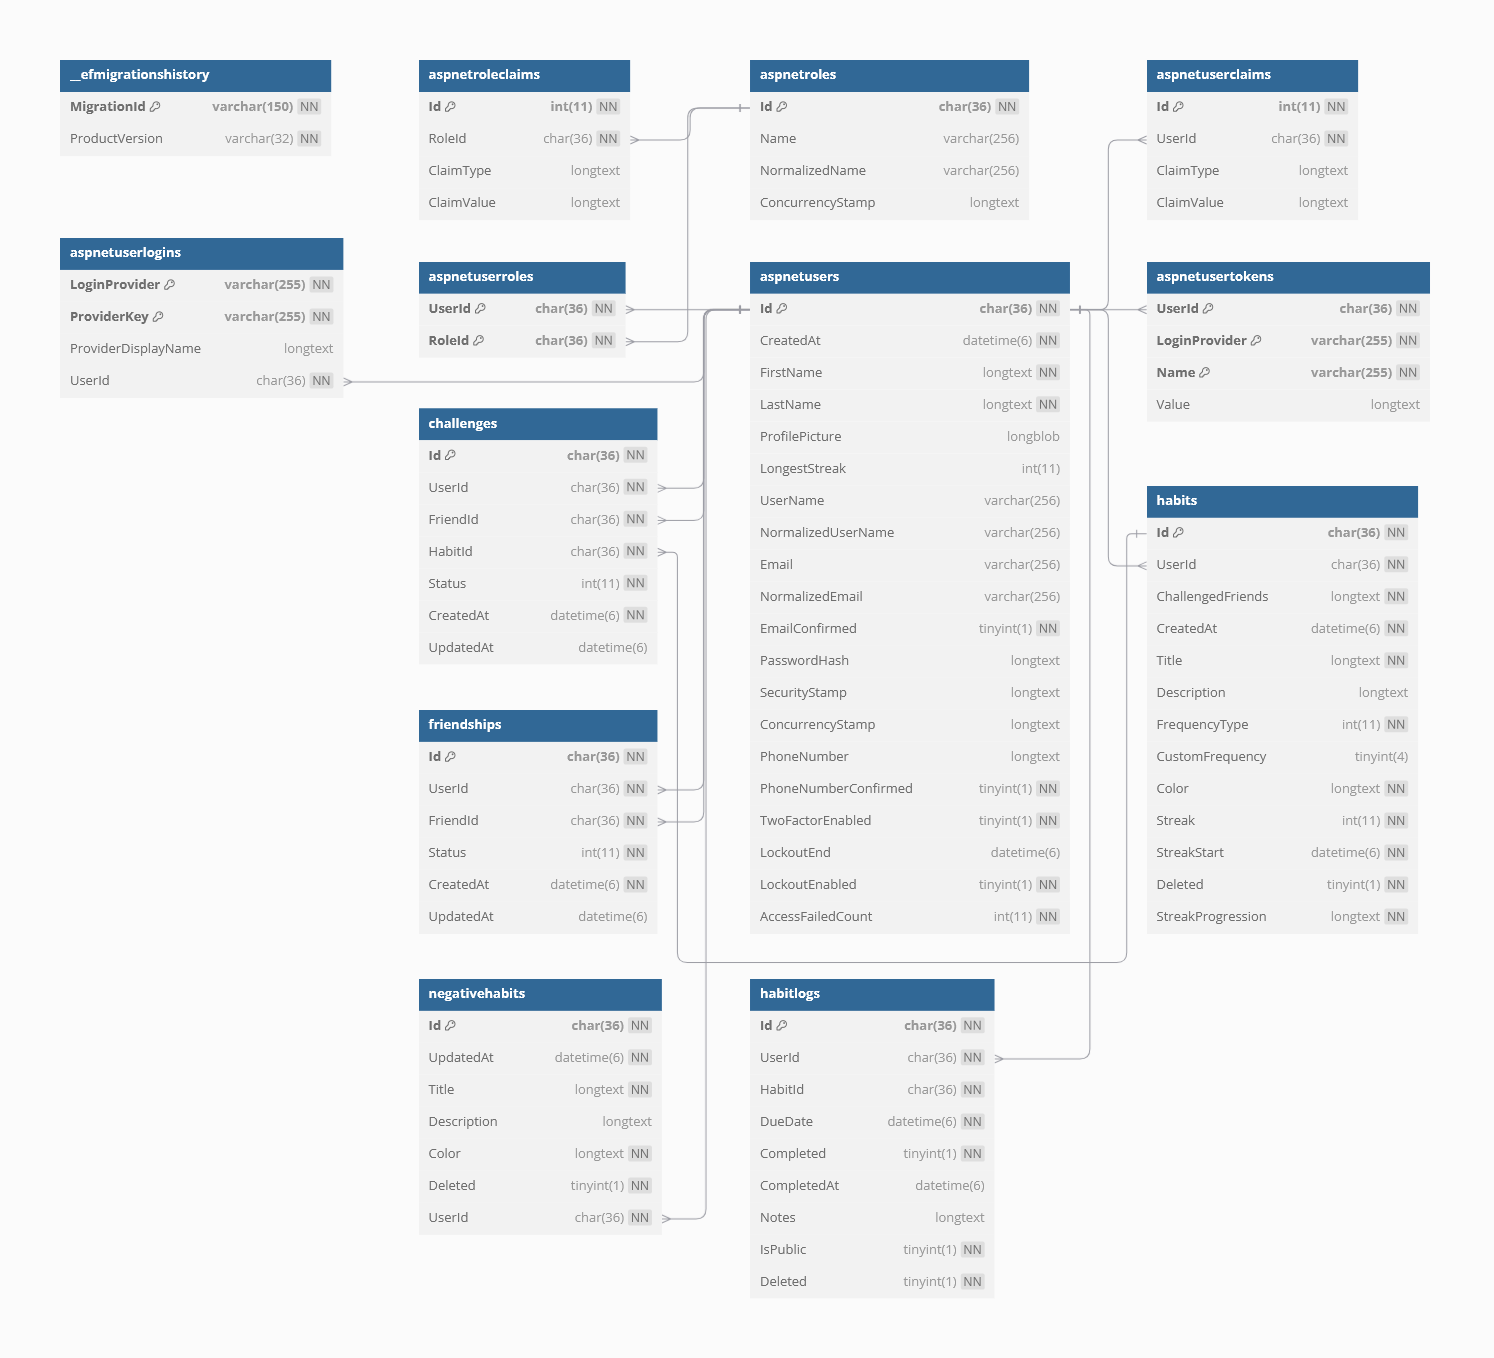
\includegraphics[width=0.8\textwidth, height=0.8\textheight, keepaspectratio]{src/diagram_full.png}
\end{figure}

\section{Adatbázis biztonság}
\begin{itemize}
  \item A jelszavak hash-elve tárolódnak az adatbázisban (ASP.NET Core Identity)
  \item Adatbázis migrációk verziókövető rendszerben tárolva
  \item A kapcsolatok integritása constraint-ekkel biztosítva
  \item Indexek használata a gyakori lekérdezések optimalizálására
\end{itemize}

\section{Adatbázis elérés}
Az adatbázis elérését a DbConnectionManager osztály biztosítja az alábbi módon:
\begin{codeblock}{DbConnectionManager.cs}
  \inputminted[
    style=one-dark,
    breaklines,
    linenos,
    firstline=24,
    lastline=38,
    gobble=8
    ]{csharp}{/home/smapesz/code/elevate/Backend/Elevate.Data/Database/DbConnectionManager.cs}
\end{codeblock}

Majd az így kapott kapcsolattal a DbContext osztály alkot egy, a későbbiekben feldolgozható adatszerkezetet.
\begin{codeblock}{ElevateDbContext.cs}
  \inputminted[
    style=one-dark,
    breaklines,
    linenos,
    firstline=61,
    lastline=86,
    gobble=8
    ]{csharp}{/home/smapesz/code/elevate/Backend/Elevate.Data/Database/ElevateDbContext.cs}
\end{codeblock} 

\chapter{Backend}

\section{Technológia}
Az Elevate backend rendszere ASP.NET Core alapú, Entity Framework Core ORM-mel. Az adatbázis és a backend kapcsolata model first elv alapján lett létrehozva. Az API RESTful elvek alapján lett kialakítva és a CRUD (Create, Read, Update, Delete) műveleteket valósítja meg.

\section{Architektúra}
A backend a következő komponensekből épül fel:
\begin{itemize}
  \item \textbf{Modellek} - Az adatmodelleket és adatbázis entitásokat reprezentálják
  \item \textbf{DTO-k (Data Transfer Objects)} - Adatok átvitelére szolgáló objektumok a rétegek között, illetve a kliens és szerver között
  \item \textbf{Repository-k} - Az adatbázissal való kommunikációért felelősek, CRUD műveletek végrehajtása
  \item \textbf{Kontrollerek} - A kérések feldolgozása, autentikáció és authorizáció kezelése, valamint a válaszok generálása
  \item \textbf{Service-k} - Az üzleti logika megvalósítása
  \item \textbf{Middleware} - Kivételek kezelése és egyéb előfeldolgozási feladatok
  \item \textbf{Segédosztályok} - Általános funkciók és segédszolgáltatások
\end{itemize}

\section{Végpontok}
A Backend API részletes dokumentációja a \href{https://elevate.koyeb.app/swagger}{\textcolor{blue}{\underline{Swagger}}} felületen érhető el. Az alábbiakban a főbb végpontok láthatóak:

\subsection{Autentikáció}
  \begin{itemize}
    \item Regisztráció (\httpPost{/api/auth/register})
    \item Bejelentkezés (\httpPost{/api/auth/login})
  \end{itemize}
\subsection{Felhasználó}
  \begin{itemize}
    \item Felhasználó adatainak lekérése email alapján (\httpGet{/api/user})
    \item Felhasználó adatainak lekérése id alapján (\httpGet{/api/user/:id})
    \item Felhasználó adatainak frissítése (\httpPatch{/api/user/:id})
  \end{itemize}
\subsection{Szokások}
  \begin{itemize}
    \item Szokások listázása (\httpGet{/api/habit})
    \item Szokás lekérése azonosító alapján (\httpGet{/api/habit/:id})
    \item Új szokás létrehozása (\httpPost{/api/habit})
    \item Szokás módosítása (\httpPatch{/api/habit/:id})
    \item Szokás törlése (\httpDelete{/api/habit/:id})
    \item Negatív szokások listázása (\httpGet{/api/habit/negative/:userId})
    \item Negatív szokás léztrehozása (\httpPost{/api/habit/negative})
    \item Negatív szokás módosítása (\httpPatch{/api/habit/negative/:id})
    \item Negatív szokás törlése (\httpDelete{/api/habit/negative/:id})
  \end{itemize}
\subsection{Szokás napló}
  \begin{itemize}
    \item Szokás naplók listázása (\httpGet{/api/habitlog})
    \item Szokás napló lekérése azonosító alapján (\httpGet{/api/habitlog/:id})
    \item Napi szokás naplók lekérése (\httpGet{/api/habitlog/:dueDate})
    \item Szokás napló frissítése (\httpPatch{/api/habitlog/:id})
  \end{itemize}
\subsection{Kihívások}
  \begin{itemize}
    \item Kihívások lekérése felhasználó azonosító alapján (\httpGet{/api/challenge/:userId/challenges})
    \item Kihívás meghívók listázása (\httpGet{/api/challenge/:userId/challenge-invites})
    \item Elküldött kihívás meghívók listázása (\httpGet{/api/challenge/:userId/sent-challenge-invites})
    \item Új kihívás létrehozása (\httpPost{/api/challenge})
    \item Kihívás státuszának frissítése (\httpPatch{/api/challenge})
    \item Kihívás törlése (\httpDelete{/api/challenge})
  \end{itemize}
\subsection{Feed}
  \begin{itemize}
    \item Feed bejegyzések lekérése (\httpGet{/api/feed})        
  \end{itemize}
\subsection{Barátok}
  \begin{itemize}
    \item Barátok listázása (\httpGet{/api/friendship/:userId/friends})
    \item Beérkezett barátkérések lekérése (\httpGet{/api/friendship/:userId/fried-requests})
    \item Küldött barátkérések lekérése (\httpGet{/api/friendship/:userId/friend-requests-sent})
    \item Barátkérés küldése (\httpPost{/api/friendship})
    \item Barátkérés elfogadása/elutasítása (\httpPatch{/api/friendship})
    \item Barátság törlése (\httpDelete{/api/friendship})
\end{itemize}

\section{Autentikáció és biztonság}
Az API biztonságos használatához JWT (JSON Web Token) alapú autentikáció van implementálva. A működése:
\begin{itemize}
  \item A felhasználó bejelentkezéskor egy JWT tokent kap(aszimmetrikus titkosítással)
  \item A token érvényességi ideje korlátozott
  \item A védett végpontok eléréséhez a tokent minden kérés fejlécében el kell küldeni
\end{itemize}

A biztonság további rétegei:
\begin{itemize}
  \item Input validáció
  \item CORS védelem (A mobil alkalmazás miatt enyhített)
  \item Jelszó titkosítás
\end{itemize}
\chapter{Tesztelés}
\section{Weboldal tesztelése}
A frontend tesztelése Cypress segítségével történt. A tesztek célja a helyes működés és a validációk biztosítása.

\subsection{Bejelentkezési oldal tesztek (\texttt{login.spec.ts})}

\begin{itemize}
  \item \textbf{Sikeres bejelentkezés} – Érvényes e-mail és jelszó megadása esetén a rendszer beenged.
  \item \textbf{Hiányzó e-mail mező} – A mező üresen hagyása validációs hibaüzenetet eredményez.
  \item \textbf{Hiányzó jelszó mező} – A mező üresen hagyása validációs hibaüzenetet eredményez.
  \item \textbf{Helytelen e-mail formátum} – Hibás e-mail formátum esetén megjelenik a validációs hiba.
  \item \textbf{Jelszó megjelenítésének váltása} – A szem ikonra kattintva a jelszó láthatóvá válik.
  \item \textbf{Navigáció a jelszó-emlékeztető oldalra} – Az „Elfelejtetted a jelszavad?” link megfelelő oldalra irányít.
  \item \textbf{Navigáció a regisztrációs oldalra} – A „Fiók létrehozása” gombra kattintva a regisztrációs oldalra navigál a felhasználó.
\end{itemize}

\subsection{Fiók létrehozása oldal tesztek (\texttt{create-account.spec.ts})}

\begin{itemize}
  \item \textbf{Sikeres fiók létrehozása} – Minden mező helyes kitöltése esetén a rendszer 201-es választ ad.
  \item \textbf{Üres mezők esetén hibaüzenet} – A regisztrációs mezők üresen hagyása validációs hibákat okoz.
  \item \textbf{Hibás e-mail formátum} – Érvénytelen e-mail cím esetén hibaüzenet jelenik meg.
  \item \textbf{Nem egyező jelszavak} – A két jelszó eltérése esetén figyelmeztetés jelenik meg.
  \item \textbf{Jelszó láthatóság kapcsolása} – A szem ikon funkcióját teszteli.
  \item \textbf{Visszatérés a bejelentkezési oldalra} – A vissza gombra kattintva a login oldalra navigálás történik.
\end{itemize}
\subsection{Dashboard oldal tesztek (\texttt{task-view.cy.ts})}

\begin{itemize}
  \item \textbf{Dátum helyes megjelenítése} – Ellenőrzi, hogy az aktuális nap dátuma helyesen jelenik meg a felületen, a hét napja és a hónap/nap formátumban.
  \item \textbf{Új feladat hozzáadási űrlap megnyitása és bezárása} – Teszteli, hogy az „Új feladat hozzáadása” gombra kattintva megjelenik az űrlap, majd az űrlap bezárására szolgáló ikonra kattintva eltűnik.
  \item \textbf{Előző nap gomb inaktívvá tétele mai nap esetén} – Ellenőrzi, hogy az előző napra léptető gomb nem elérhető (le van tiltva) ha az aktuális dátumot nézzük.
  \item \textbf{„Nincs feladat mára” üzenet megjelenése} – Szimulált adat hiányában ellenőrzi, hogy megjelenik a „Nincs feladat mára!” és a „Kattints az 'Add' gombra új szokás létrehozásához.” szöveg.
  \item \textbf{Pozitív szokás létrehozása} – Teszteli, hogy egy új pozitív szokást helyesen lehet hozzáadni: cím, leírás, szín és gyakoriság megadásával.
\end{itemize}
\subsection{Barátok oldal tesztek (\texttt{friends-page.cy.ts})}

\begin{itemize}
  \item \textbf{Betöltési animáció megjelenése barátok lekérése közben} – Teszteli, hogy az adatok betöltése során a spinner látható.
  \item \textbf{Üzenet megjelenése, ha nincsenek barátok} – Ellenőrzi, hogy ha nincs visszaküldött barát adat, akkor egy „nincsenek barátaid” üzenet jelenik meg.
  \item \textbf{Barátok listájának megjelenítése} – Valós adatok esetén ellenőrzi, hogy a barátok neve és e-mail címe megjelenik a listában.
  \item \textbf{Barát törlése} – Teszteli, hogy egy barát törlése után a felhasználó eltűnik a listából.
  \item \textbf{Felhasználók keresése e-mail alapján} – Ellenőrzi, hogy a keresőmező segítségével megadható e-mail cím alapján megjelennek a találatok.
  \item \textbf{Barát felkérés küldése} – Teszteli, hogy a keresési találat melletti „követés” ikonra kattintva barátfelkérés küldése történik, és az ikon „elfogadva” állapotra vált.
  \item \textbf{Barátkérések megjelenítése} – Ellenőrzi, hogy a beérkező barátkérések listája helyesen jelenik meg az oldalon.
  \item \textbf{Barátkérés elfogadása} – Teszteli, hogy a beérkező barátkérés elfogadása után az adott kérés eltűnik a listából.
  \item \textbf{Barátkérés elutasítása} – Teszteli, hogy a barátkérés elutasítása után az adott kérés eltűnik a listából.
\end{itemize}

\section{Unit tesztelés}
A backend tesztelésére az xUnit keretrendszert használtuk, amellyel a Service réteg metódusait teszteltük mockolt adatokkal. 

\begin{figure}[H]
    \centering
    \begin{minipage}[b]{0.3\textwidth}
        \centering
        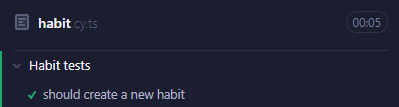
\includegraphics[width=\linewidth]{src/habittest.png}
        \caption{Első kép}
        \label{fig:img1}
    \end{minipage}
    \hspace{0.03\textwidth}
    \begin{minipage}[b]{0.3\textwidth}
        \centering
        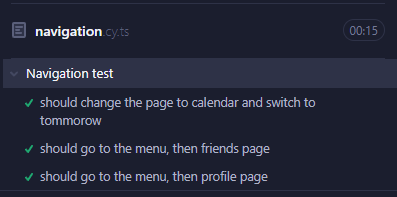
\includegraphics[width=\linewidth]{src/navigationtest.png}
        \caption{Második kép}
        \label{fig:img2}
    \end{minipage}
    \hspace{0.03\textwidth}
    \begin{minipage}[b]{0.3\textwidth}
        \centering
        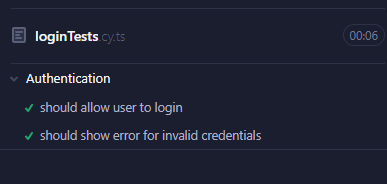
\includegraphics[width=\linewidth]{src/logintest.png}
        \caption{Harmadik kép}
        \label{fig:img3}
    \end{minipage}
\end{figure}

A fenti képeken a Cypress által végrehajtott end-to-end tesztek láthatók, amelyek ellenőrzik az alkalmazás különböző funkcióinak működését. A tesztelés során ellenőriztük a felhasználói bejelentkezést, az adatbevitel validációját és az egyes oldalak közötti navigációt is.

\chapter{Használati útmutató mobilhoz}
\section{Login}
A következő képernyőképek a mobilos bejelentkezési folyamat lépéseit mutatják be:

\begin{figure}[H]
    \centering
    \begin{minipage}[b]{0.23\textwidth}
        \centering
        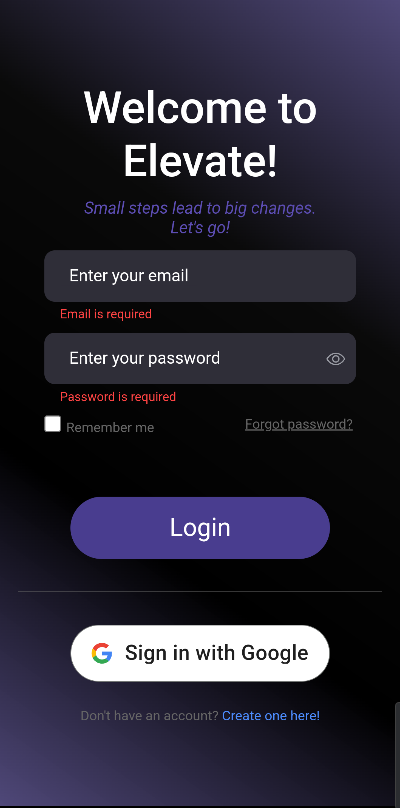
\includegraphics[width=\linewidth]{src/loginpage1.png}
       1. lépés
    \end{minipage}
    \hfill
    \begin{minipage}[b]{0.23\textwidth}
        \centering
        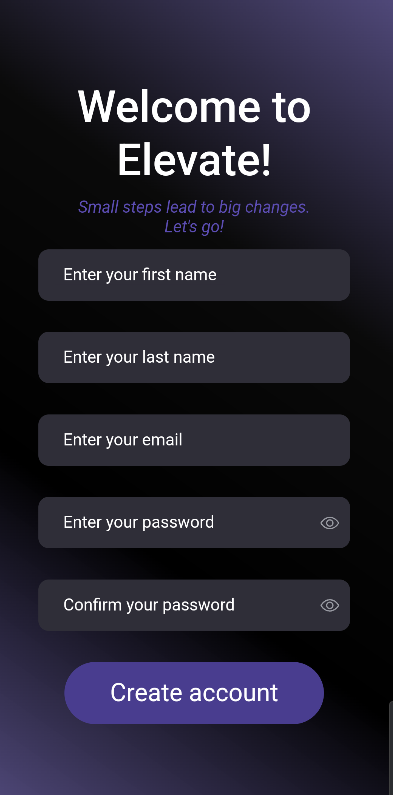
\includegraphics[width=\linewidth]{src/loginpage2.png}
       2. lépés
    \end{minipage}
    \hfill
    \begin{minipage}[b]{0.23\textwidth}
        \centering
        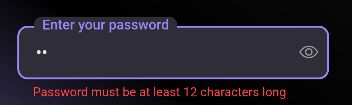
\includegraphics[width=\linewidth]{src/loginpage3.png}
        3. lépés
    \end{minipage}
    \hfill
    \begin{minipage}[b]{0.23\textwidth}
        \centering
        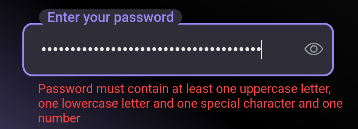
\includegraphics[width=\linewidth]{src/loginpage4.png}
        4. lépés
    \end{minipage}
   Mobilos bejelentkezés lépései
    \label{fig:login-steps}
\end{figure}

Amennyiben a felhasználó nem rendelkezik fiókkal, meg kell nyomnia a Create one here! gombot.  A sikeres regisztráció után automatikusan átirányítás történik a bejelntkezési oldalra, ahogy be kell jelentkezni a már meglévő fiókkal. Amennyiben a felhasználó rendelkezik fiókkal, nem kell regisztrálnia. Sikeres bejelentkezés után automatikusan átirányítás történik a Szokások (Habits) oldalra
\section{Szokás hozzáadás}
\begin{figure}[H]
    \centering

    % First row - 3 images
    \begin{minipage}[b]{0.25\textwidth}
        \centering
        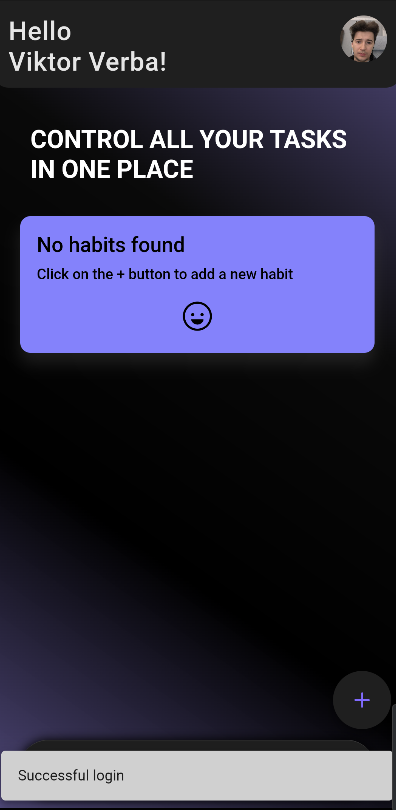
\includegraphics[width=\linewidth]{src/habit1.png}
       Szokás hozzáadása, meg kell nyomni a + gombot
    \end{minipage}
    \hfill
    \begin{minipage}[b]{0.25\textwidth}
        \centering
        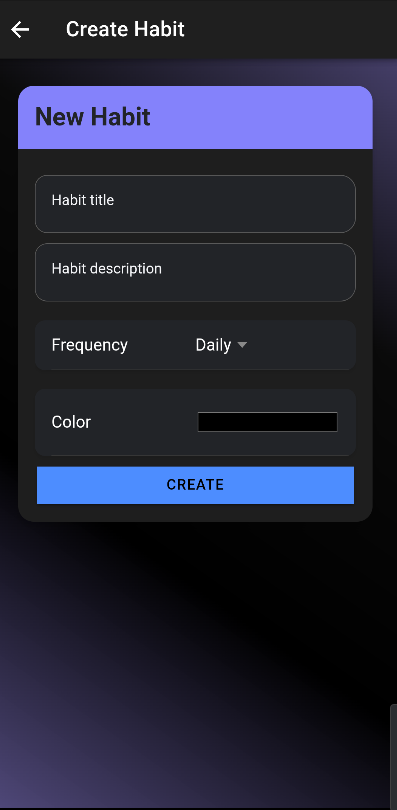
\includegraphics[width=\linewidth]{src/habit2.png}
       Szokás adatainak feltöltése
    \end{minipage}
    \hfill
    \begin{minipage}[b]{0.25\textwidth}
        \centering
        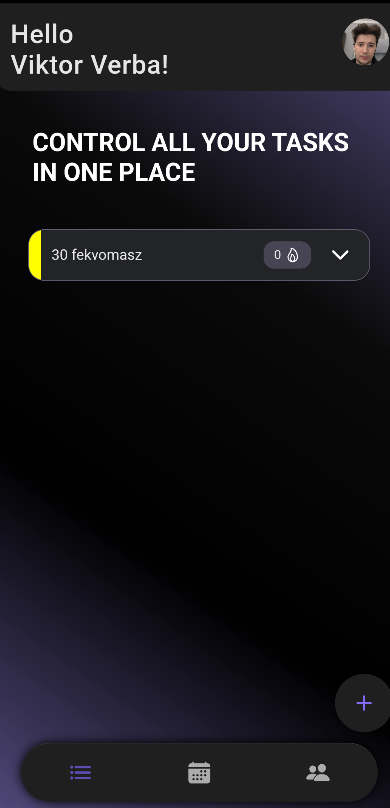
\includegraphics[width=\linewidth]{src/habit3.png}
        Láthatjuk a frissen hozzáadott szokást
    \end{minipage}

    \vspace{0.8em}

    % Second row - 2 images
    \hfill
    \begin{minipage}[b]{0.25\textwidth}
        \centering
        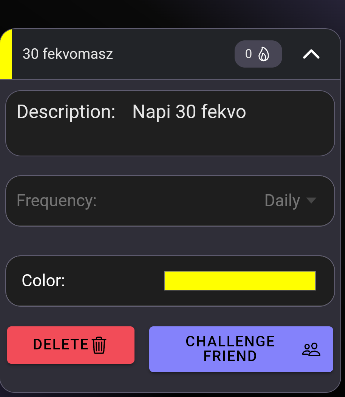
\includegraphics[width=\linewidth]{src/habitkinyilt.png}
        Kattintásra kinyílik a szokás
    \end{minipage}

    {Szokás létrehozásának lépései a mobilalkalmazásban}
    \label{fig:habit-creation}
\end{figure}

A fenti képeken látható, hogyan lehet egy új szokást hozzáadni az alkalmazáson belül. A felhasználó kiválasztja a szokás típusát, megadja a nevet, gyakoriságot, majd elmenti azt. Ez segít abban, hogy a napi célkitűzések következetesen teljesüljenek.

\section{Szokás teljesítés}
\begin{figure}[H]
    \centering

    \begin{minipage}[b]{0.3\textwidth}
        \centering
        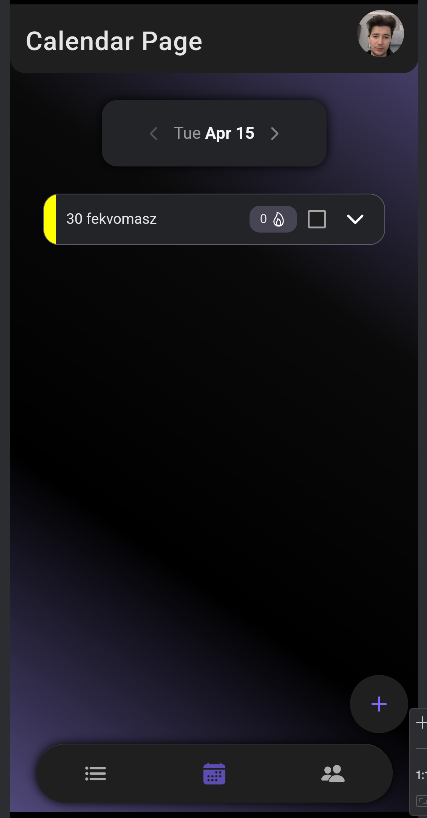
\includegraphics[width=\linewidth]{src/habitdone1.png}
       Napi nézett, kis kockára kattintva teljesíthető a szokás
    \end{minipage}
    \hfill
    \begin{minipage}[b]{0.3\textwidth}
        \centering
        
\includegraphics[width=\linewidth]{src/habitdone2.png}
        Kiválasztás hogy publikus legyen-e a teljesítésünk
    \end{minipage}
    \hfill
    \begin{minipage}[b]{0.3\textwidth}
        \centering
        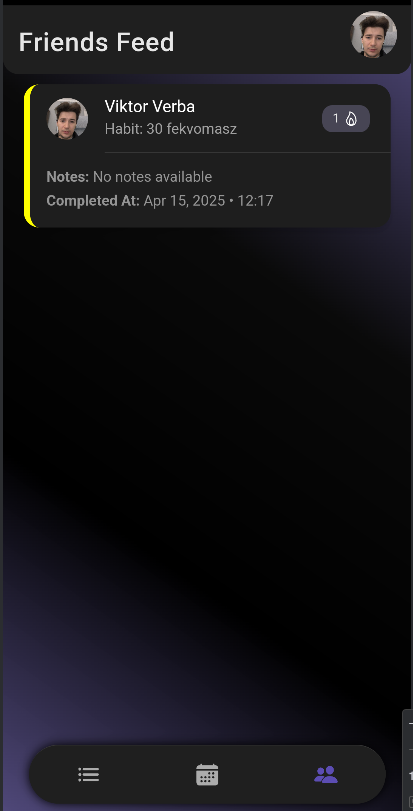
\includegraphics[width=\linewidth]{src/habitdone3.png}
        Amennyiben publikusat választottunk, a szokás megjelenik a feed oldalon
    \end{minipage}

\end{figure}
  A fenti lépések bemutatják, hogyan lehet egy szokást teljesítettként jelölni a naptár nézetben és megjeleniteni feed-ben. Kalendár nézetben válthatjuk a napokat nyílak segítségével. 

\section{Barátok hozzáadása}
\begin{figure}[H]
    \centering

    % Első sor - 3 kép
    \begin{minipage}[b]{0.25\textwidth}
        \centering
        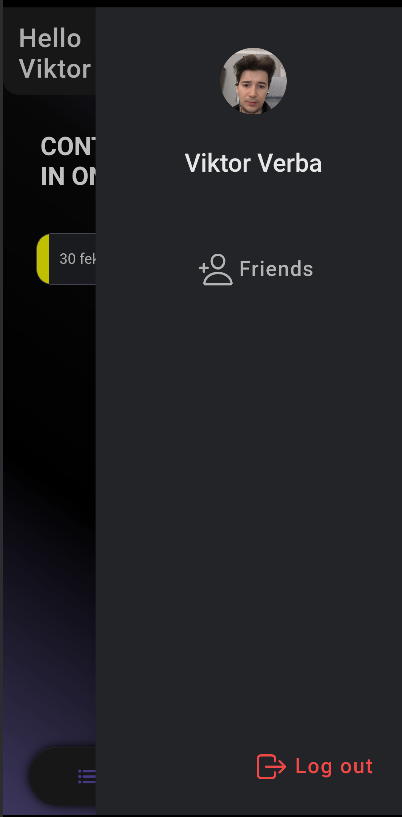
\includegraphics[width=\linewidth]{src/friends1.png}

    \end{minipage}
    \hfill
    \begin{minipage}[b]{0.25\textwidth}
        \centering
        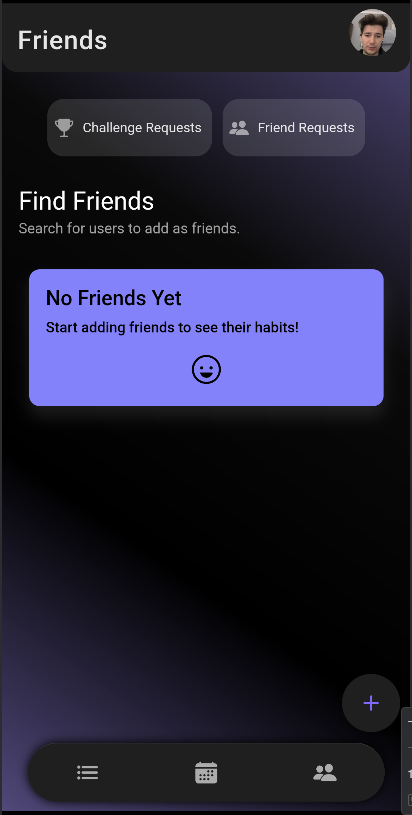
\includegraphics[width=\linewidth]{src/friends2.png}

    \end{minipage}
    \hfill
    \begin{minipage}[b]{0.25\textwidth}
        \centering
        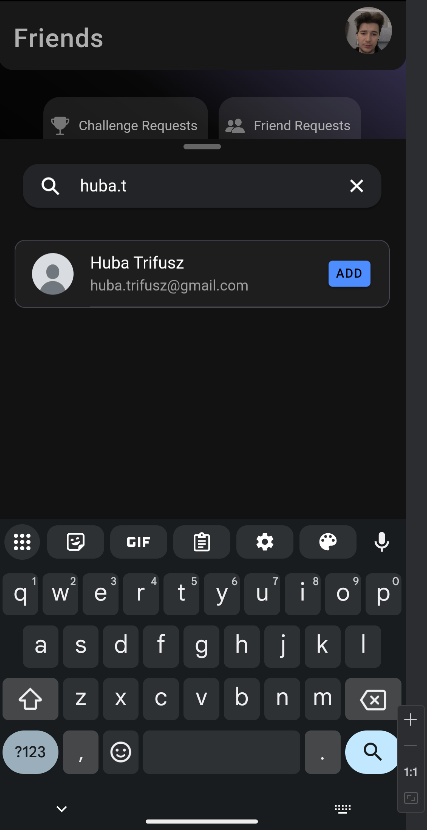
\includegraphics[width=\linewidth]{src/friends3.png}

    \end{minipage}

    \vspace{0.8em} % Kis függőleges térköz a sorok között

    % Második sor - 2 kép
    \begin{minipage}[b]{0.25\textwidth}
        \centering
        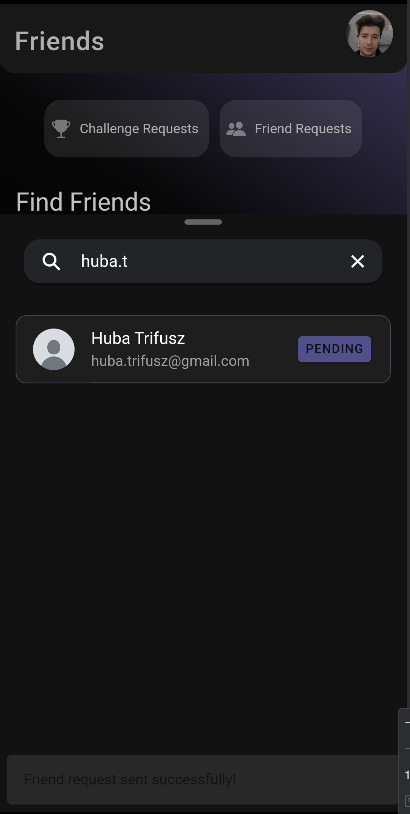
\includegraphics[width=\linewidth]{src/friends4.png}

    \end{minipage} % Üres hely a középső pozícióra
    \begin{minipage}[b]{0.25\textwidth}
        \centering
        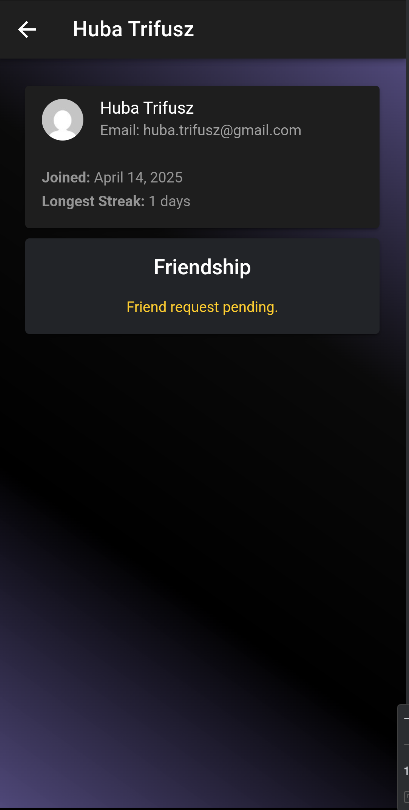
\includegraphics[width=\linewidth]{src/friends5.png}

    \end{minipage}

\end{figure}

    Profileképre kattintva megjelenik a menü, ahogy Friends gombra kattintva átírányit minket a program Barátok oldalra. Itt láthatjuk hogy nincs barátunk, + gombra kattintva kereshetünk a felhasználók között. Miután megtaláltunk a keresett személyt rákattinthatunk az Add gombra.         Miután megnyomtunk a gomb felírata megváltozik. Keresett felhasználó profilképére kattintva megtekinthetjuk a felhasználó összes adatát és azt is hogy a baráti kérelem el lett küldve.

\section{Baráti kérelem fogadás}
\begin{figure}[H]
    \centering

    % Felső sor - 3 kép
    \begin{minipage}[t]{0.25\textwidth}
        \centering
        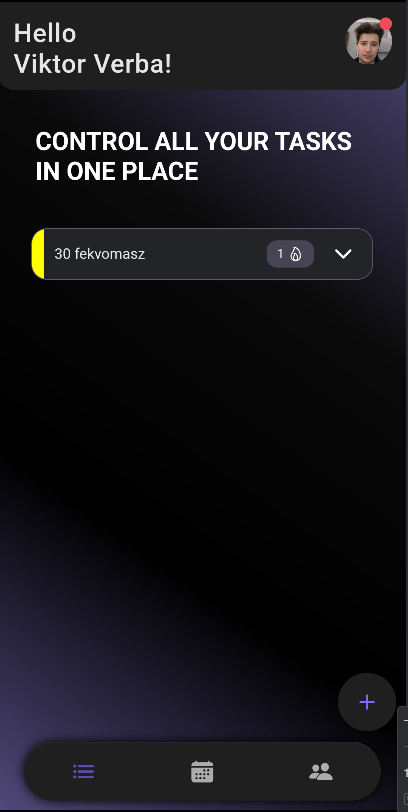
\includegraphics[width=\linewidth]{src/friendrequest1.png}
    \end{minipage}
    \hfill
    \begin{minipage}[t]{0.25\textwidth}
        \centering
        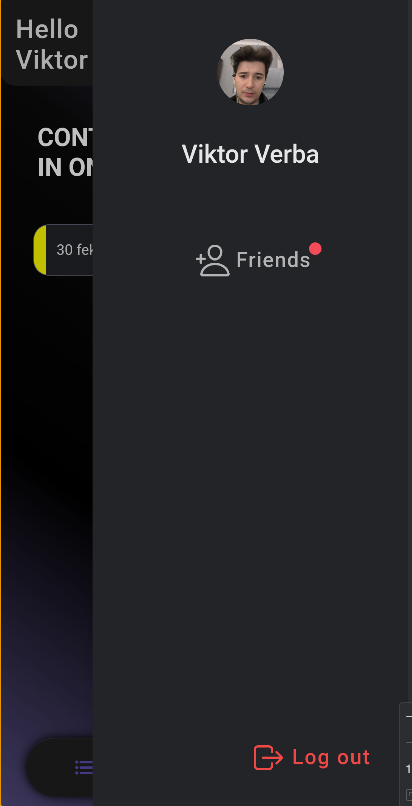
\includegraphics[width=\linewidth]{src/friendrequest2.png}
    \end{minipage}
    \hfill
    \begin{minipage}[t]{0.25\textwidth}
        \centering
        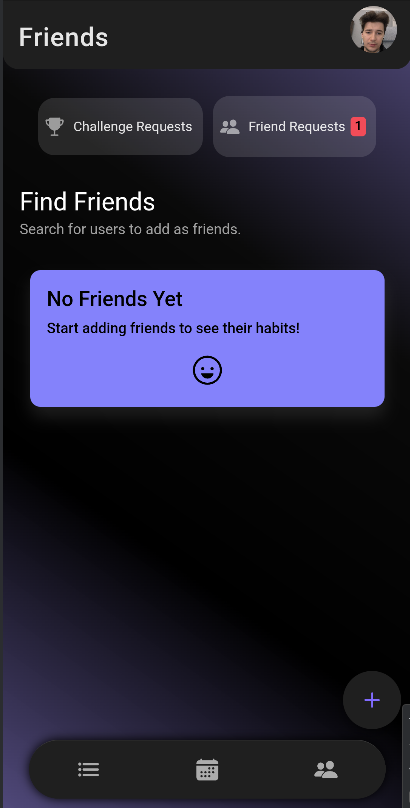
\includegraphics[width=\linewidth]{src/friendrequest3.png}
    \end{minipage}

    \vspace{0.8em}

    % Alsó sor - 2 kép
    \begin{minipage}[t]{0.25\textwidth}
        \centering
        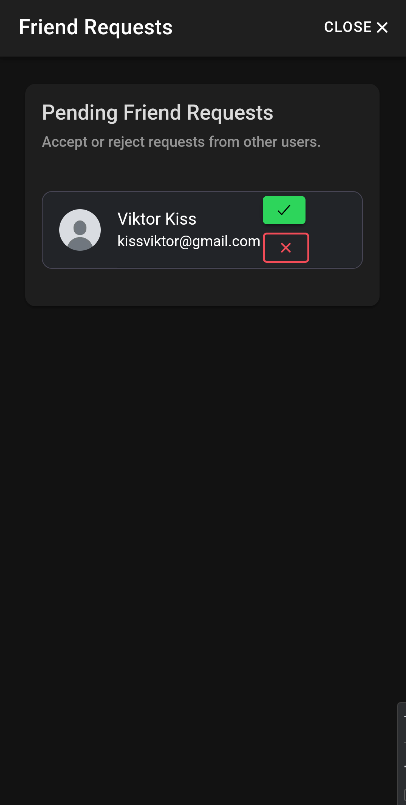
\includegraphics[width=\linewidth]{src/friendrequest4.png}
    \end{minipage}
    \hfill
    \begin{minipage}[t]{0.25\textwidth}
        \centering
        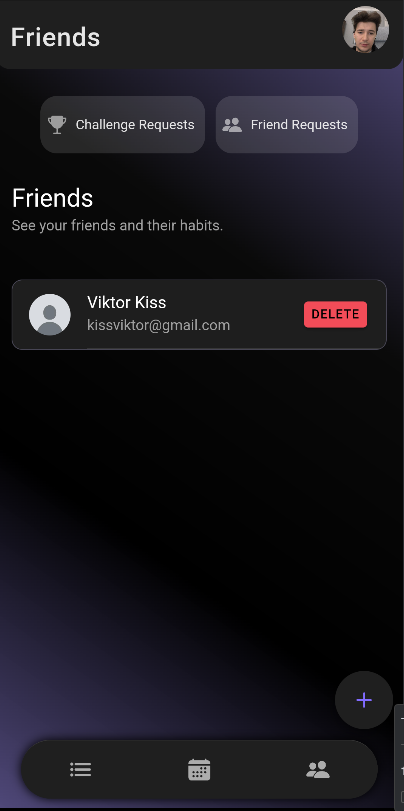
\includegraphics[width=\linewidth]{src/friendrequest5.png}
    \end{minipage}

\end{figure}
  Amennyiben a program észlel, hogy valaki küldött nekünk baráti kérelmet vagy challenge kérelmet a profilképnél megjeleník egy kis piros pötty. Miután rákattintunk a profilképünkre a Friends gombon is látni fogjuk a pöttyöt, ami azt jelzi, hogy ezen az oldalon érkezett kérelem. Miután barátok oldalra lépünk láthatjuk a baráti kérelem és challenge gombokat. Piros szám azt jelzi hogy hány kérelem érkezett hozzánk. Friend Requests gombra kattintva megjelennek a beérkezett baráti kérelmek. Elfogadás után a barátunk megjelenik a listában.
\section{Kihívás}
% Első oldal - 6 kép
\begin{figure}[H]
    \centering

    % 1. sor
    \begin{minipage}[b]{0.25\textwidth}
        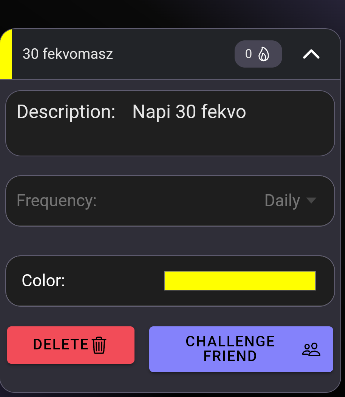
\includegraphics[width=\linewidth]{src/habitkinyilt.png}
    \end{minipage}
    \hfill
    \begin{minipage}[b]{0.25\textwidth}
        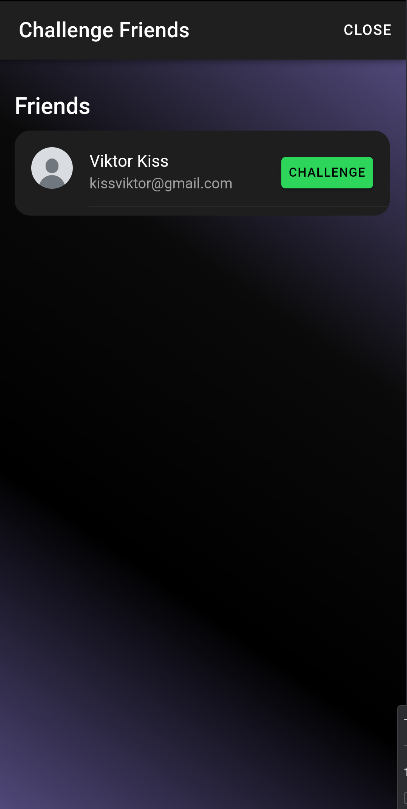
\includegraphics[width=\linewidth]{src/challenge1.png}
    \end{minipage}
    \hfill
    \begin{minipage}[b]{0.25\textwidth}
        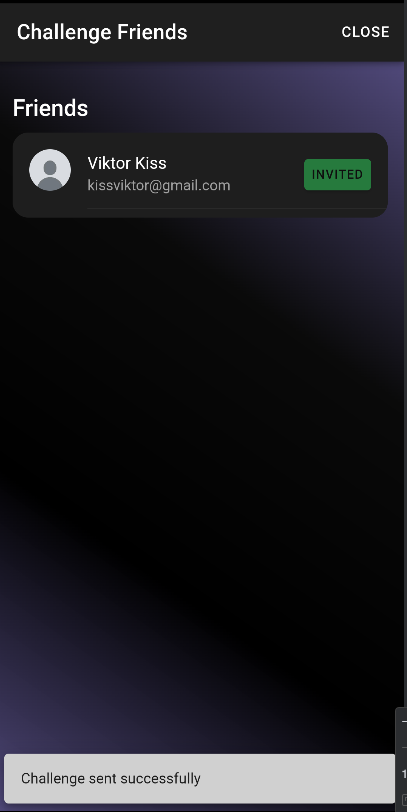
\includegraphics[width=\linewidth]{src/challenge2.png}
    \end{minipage}

    \vspace{0.8em}

    % 2. sor
    \begin{minipage}[b]{0.25\textwidth}
        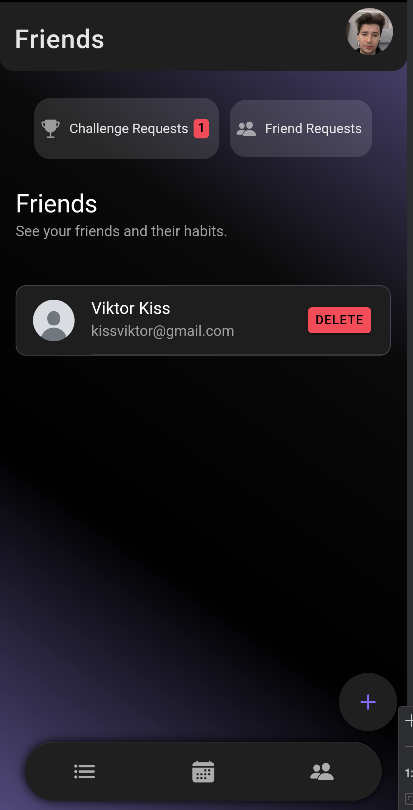
\includegraphics[width=\linewidth]{src/challenge3.png}
    \end{minipage}
    \hfill
    \begin{minipage}[b]{0.25\textwidth}
        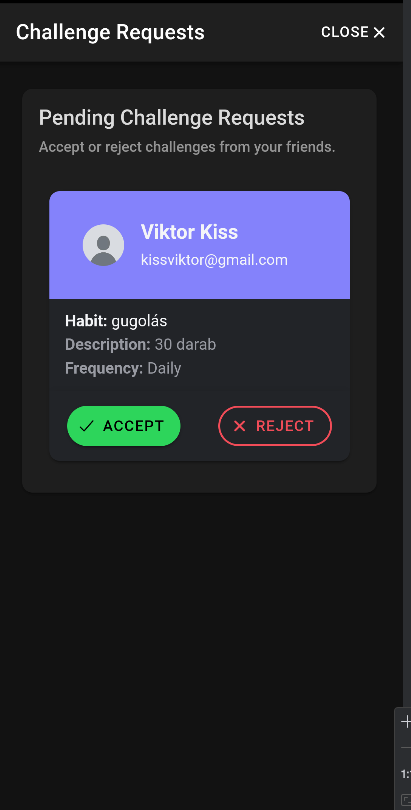
\includegraphics[width=\linewidth]{src/challenge4.png}
    \end{minipage}
    \hfill
    \begin{minipage}[b]{0.25\textwidth}
        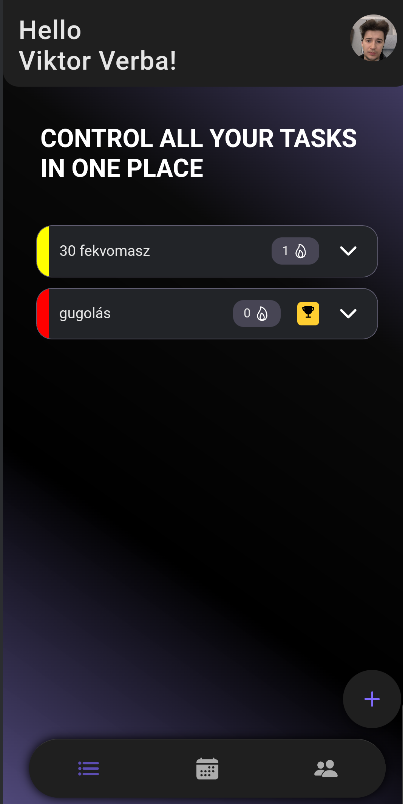
\includegraphics[width=\linewidth]{src/challenge5.png}
    \end{minipage}
\end{figure}

\newpage

% Második oldal - 3 kép
\begin{figure}[H]
    \centering

    % 3. sor
    \begin{minipage}[b]{0.3\textwidth}
        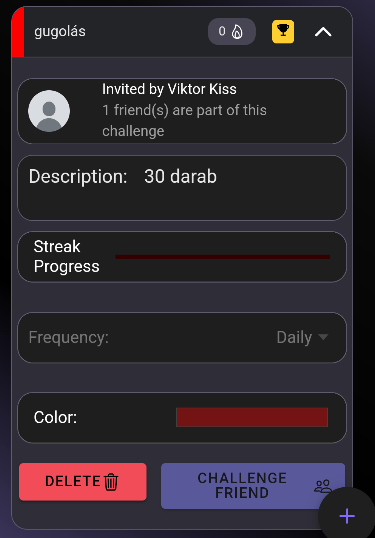
\includegraphics[width=\linewidth]{src/challenge6.png}
    \end{minipage}
    \hfill
    \begin{minipage}[b]{0.3\textwidth}
        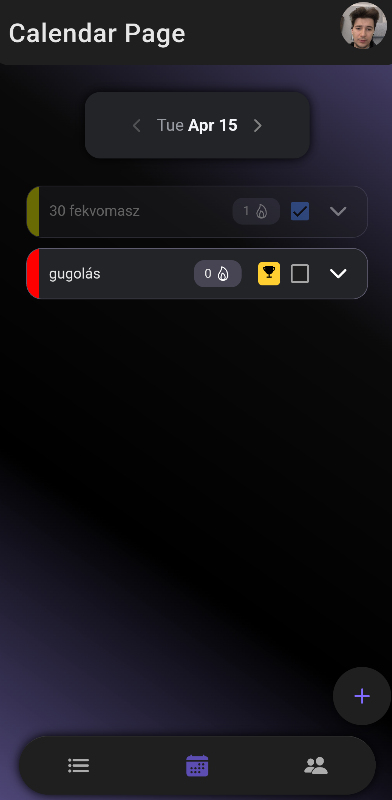
\includegraphics[width=\linewidth]{src/challenge7.png}
    \end{minipage}
    \hfill
    \begin{minipage}[b]{0.3\textwidth}
        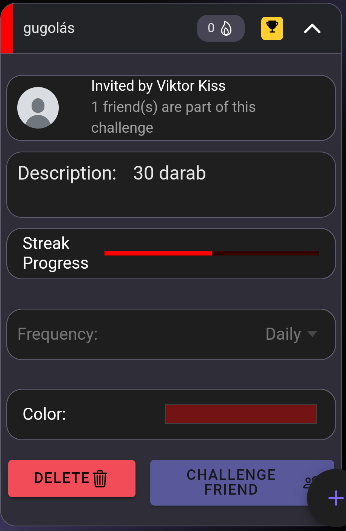
\includegraphics[width=\linewidth]{src/challenge8.png}

    \end{minipage}
\end{figure}
    \footnotesize Amennyiben a felhasználó rendelkezik barátokkal, akkor tud küldeni a barátainak kihívást (challenget) amit onnantól közösen kell elvégezniuk ahhoz, hogy a streak nőjőn. Szokásra kattintva rá kell kattintani a Challenge friend gombra, amely átvisz egy oldalra, ahol kiválaszthatjuk a barátot, akit meg akarjuk hívni. Miután rákattintottunk a challenge gombra, kapunk visszajelzést és a gomb átváltozik Invited-re. További képeken látható, hogy kell elfogadni vagy elutasítani a kihívásokat. Amennyiben elfogadjuk a kihívást az meg fog jelenni a szokásaink közül. Kihívást egy kis ikonnal tudunk megkülönböztetni. Ha valaki meghívott minket, akkor láthatjuk ki volt az és hányan vesznek részt benne. Streak Progress mutatja, hogy eddig hányan teljesítették a resztvevők közül a kihívást.

\section{Profilkép}
\begin{figure}[H]
    \centering

    \begin{minipage}[b]{0.3\textwidth}
        \centering
        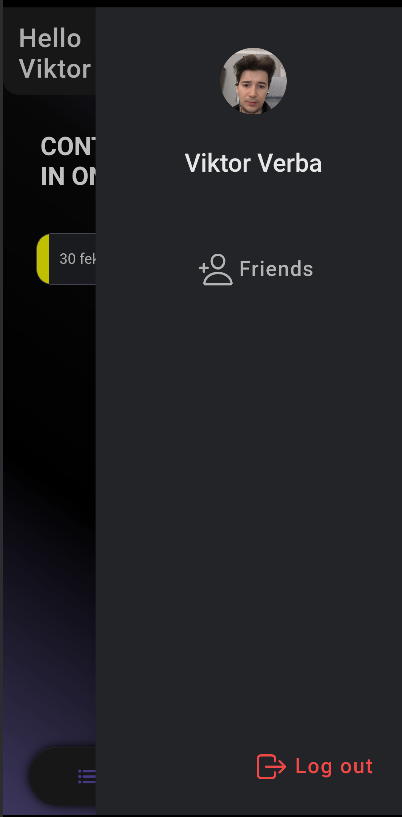
\includegraphics[width=\linewidth]{src/friends1.png}
        \par
        \footnotesize Profileképre kattintva átvisz minket a profil oldalra. 
    \end{minipage}
    \hfill
    \begin{minipage}[b]{0.3\textwidth}
        \centering
        
\includegraphics[width=\linewidth]{src/profilepic1.png}
        \par
        \footnotesize Profilképre kattintva kiválaszthatjuk, hogy képek közül akarunk választani vagy csinálni akarunk egy képet.
    \end{minipage}
    \hfill
    \begin{minipage}[b]{0.3\textwidth}
        \centering
        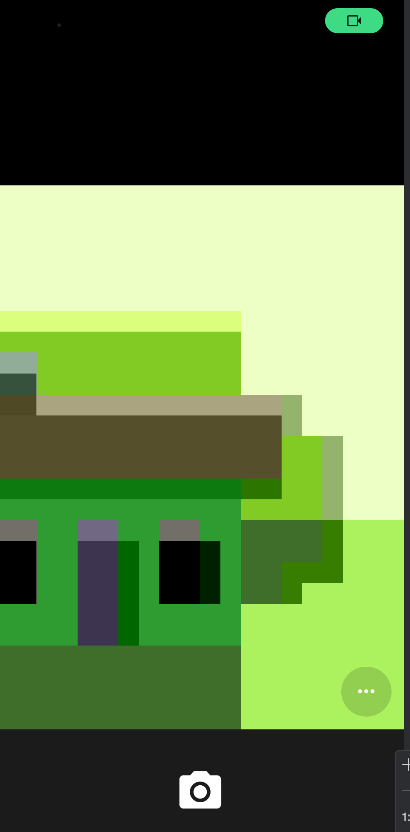
\includegraphics[width=\linewidth]{src/profilepic2.png}
        \par
        \footnotesize Képcsinálásra megnyílik a kamera
    \end{minipage}

\end{figure}
\section{Negatív szokás}
\begin{figure}[H]
    \centering
    \begin{minipage}[b]{0.2\textwidth}
        \centering
        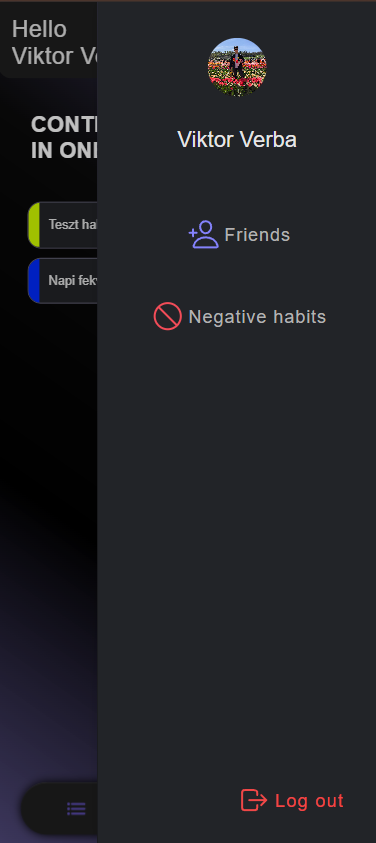
\includegraphics[width=\linewidth]{src/Oldaltmenu.png}
        \par
        \footnotesize Oldalsó menü megnyitása. Negative habits gombra kattintva megjelenik a Negative Habits oldal.
    \end{minipage}
    \hfill
    \begin{minipage}[b]{0.2\textwidth}
        \centering
        \includegraphics[width=\linewidth]{src/ÜresNegativeHAbit.png}
        \par
        \footnotesize Üres negatív szokás lista.
    \end{minipage}
    \hfill
    \begin{minipage}[b]{0.2\textwidth}
        \centering
        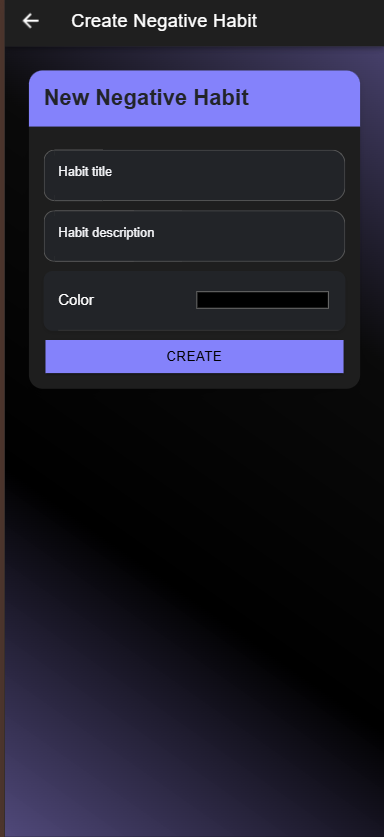
\includegraphics[width=\linewidth]{src/NegativeHozzaad.png}
        \par
        \footnotesize Új negatív szokás hozzáadása.
    \end{minipage}

    \vspace{0.8em}

    \begin{minipage}[b]{0.2\textwidth}
        \centering
        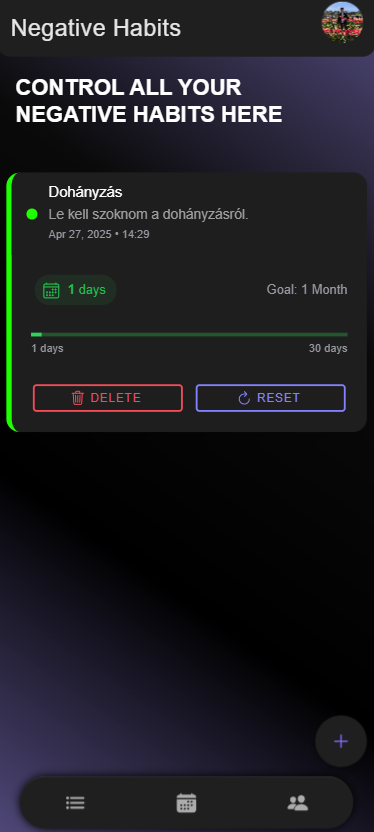
\includegraphics[width=\linewidth]{src/Negativemegjelenes.png}
        \par
        \footnotesize A negatív szokás megjelenése a listában. Plusz gombra kattintva hozzáadhatjuk egy új szokást.
    \end{minipage}
    \hfill
    \begin{minipage}[b]{0.2\textwidth}
        \centering
        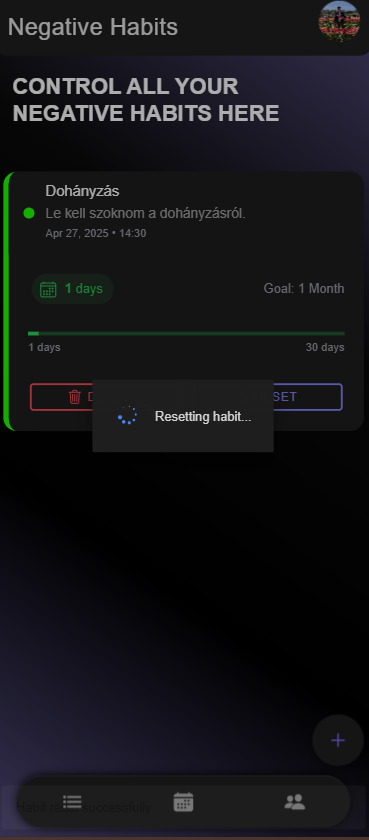
\includegraphics[width=\linewidth]{src/resetingNegativeHabit.png}
        \par
        \footnotesize Negatív szokás resetelése. Akkor használjuk mikor nem teljesitettünk egy adott fogadalmat és ezért elveszik a streak.
    \end{minipage}

\end{figure}

\chapter{Források}
\begin{itemize}
  \item \href{https://learn.microsoft.com/en-us/ef/core/}{\textcolor{blue}{\underline{Microsoft Docs - Entity Framework Core}}{ (2025.04.15.)}}
  \item \href{https://www.koyeb.com/docs}{\textcolor{blue}{\underline{Koyeb Documentation}}{ (2025.04.15.)}}
  \item \href{https://swagger.io/docs/open-source-tools/swagger-ui/usage/installation/}{\textcolor{blue}{\underline{Swagger UI Documentation}}{ (2025.04.15.)}}
\end{itemize}

\end{document}
